% !TeX root = ../thesis.tex

\chapter{System}
\label{sec:system}
In diesem Kapitel werden die einzelnen analoge Signalverarbeitungskomponenten näher erläutert und zu einem ganzen System zusammengefügt. Da hier sowohl digitale als auch Analoge Signalverarbeitungsbausteine in Einklang gebracht werden sollen, werden zunächst die Eigenschaften des analogen Schaltkreises eingegangen. Darauf folgend werden der physikalische Aufbau von Schaltung und Gehäuse, aber auch das Thermische Management des Systems thematisiert. Zudem setzt sich dieses Kapitel mit der Ansteuerung der Potentiometer auseinander, welche es dem Sender ermöglichen den Offset und die Amplitude frei zu variieren. Zuletzt werden Einstellungs- und Evaluierungsparameter der Modulationssoftware Dream für Sender und Empfänger erörtert.


\section{Analoge Signalverarbeitung}
\label{sec:Signalverarbeitung}
Bei der Signalübertragung über den optischen Kanal mit dem in dieser Abschlussarbeit gewählten Medium Licht, müssen einige grundlegende Dinge beachtet werden. Im Kapitel~\ref{sub:led} der Leuchtdiode wurden ihre grundlegenden Eigenschaften erklärt, die es sich hier nun zu verwenden gilt. Eine bekannte Schwierigkeit ist die Übertragung von negativen Wellen. Diese können nicht Übertragen werden, da Licht keinen negativen Wert annehmen kann. Hinzu ist man bei der Übertragung von Signalen darauf bedacht, nur im linearen Bereich der LED-Kennlinie Daten zu übertragen. Wenn man diese nämlich im nichtlinearen Bereich der LED Überträgt, können Verzerrungen auftreten und somit die Übertragung stark gestört werden. Um jenes Problem zu lösen, wird ein Offset verwendet, welcher das Signal so positiv verschiebt, dass dieses keine negativen Anteile mehr besitzt. Zudem wurde ein Spannungspuffer eingerichtet um zusätzlich die Amplitude zu verstärken. Dies liefert Gewissheit, dass nur positive Spannungsanteile übertragen werden und somit kein Signalverlust verzeichnet werden muss.

\begin{figure}[H]
	\centering
	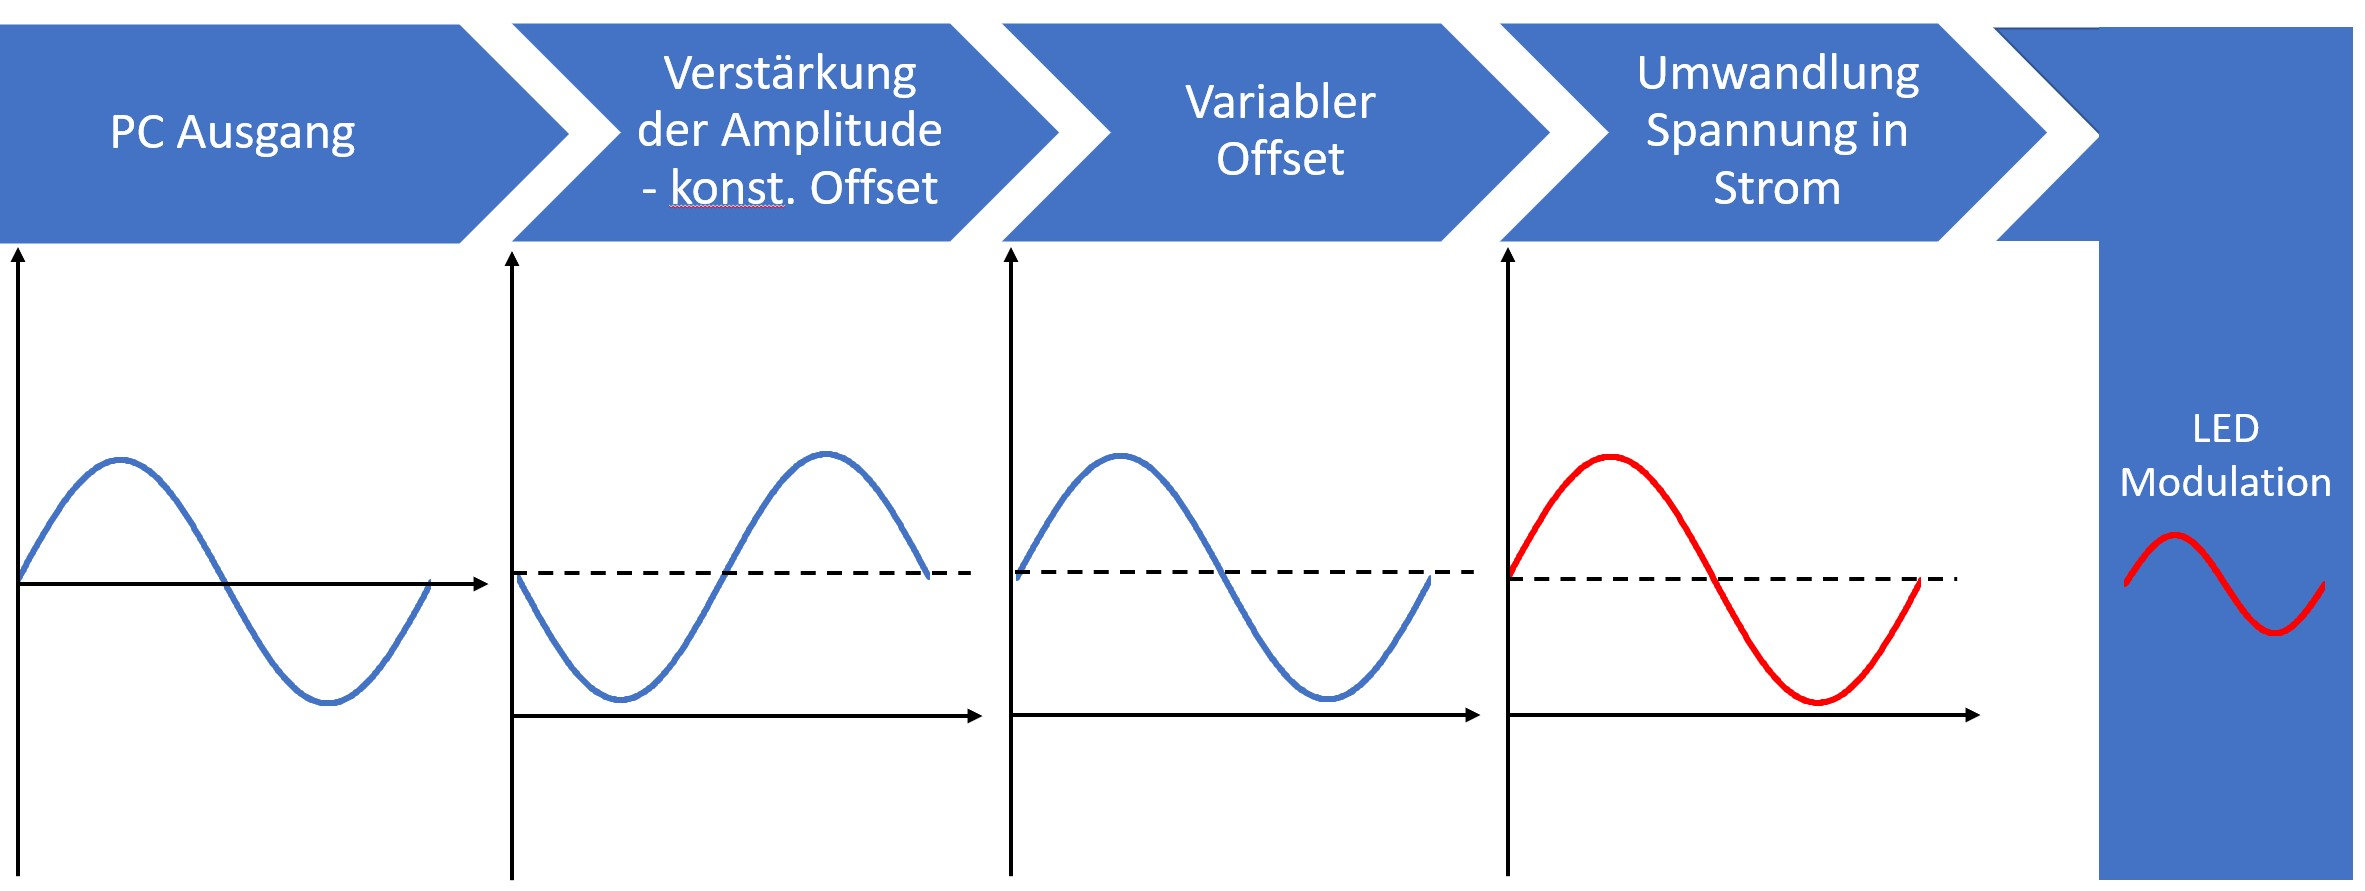
\includegraphics[width = 1 \textwidth ]{signalvorgang.jpg}
	\caption[Signalverarbeitungsschritte]{Signalverarbeitungsschritte} \gls{online:Eigen}
	\label{fig:signalvorgang}
\end{figure}

In Abbildung ~\ref{fig:signalvorgang} werden die Verschiedenen Stufen der Signalübertragung veranschaulicht. Da es sich an dieser Stelle um ein nichtlineares System handelt, dürfen die Signalverarbeitungsstufen nicht beliebig vertauscht werden. Eine solche Veränderung der Reihenfolge könnte zur Verfälschung des Signals führen. 

Die analoge Signalverarbeitungsschaltung wurde in drei Stufen aufgeteilt. Die \gls{acr:OP}- Grundschaltungen wurden hierfür so modifiziert, dass Amplitude und Offset variabel einstellbar sind und möglich auftretende Fehler vermieden werden. In Abbildung ~\ref{fig:stufe1} ist die Eingangssignalverarbeitungsstufe illustriert. 

\begin{figure}[H]
	\centering
	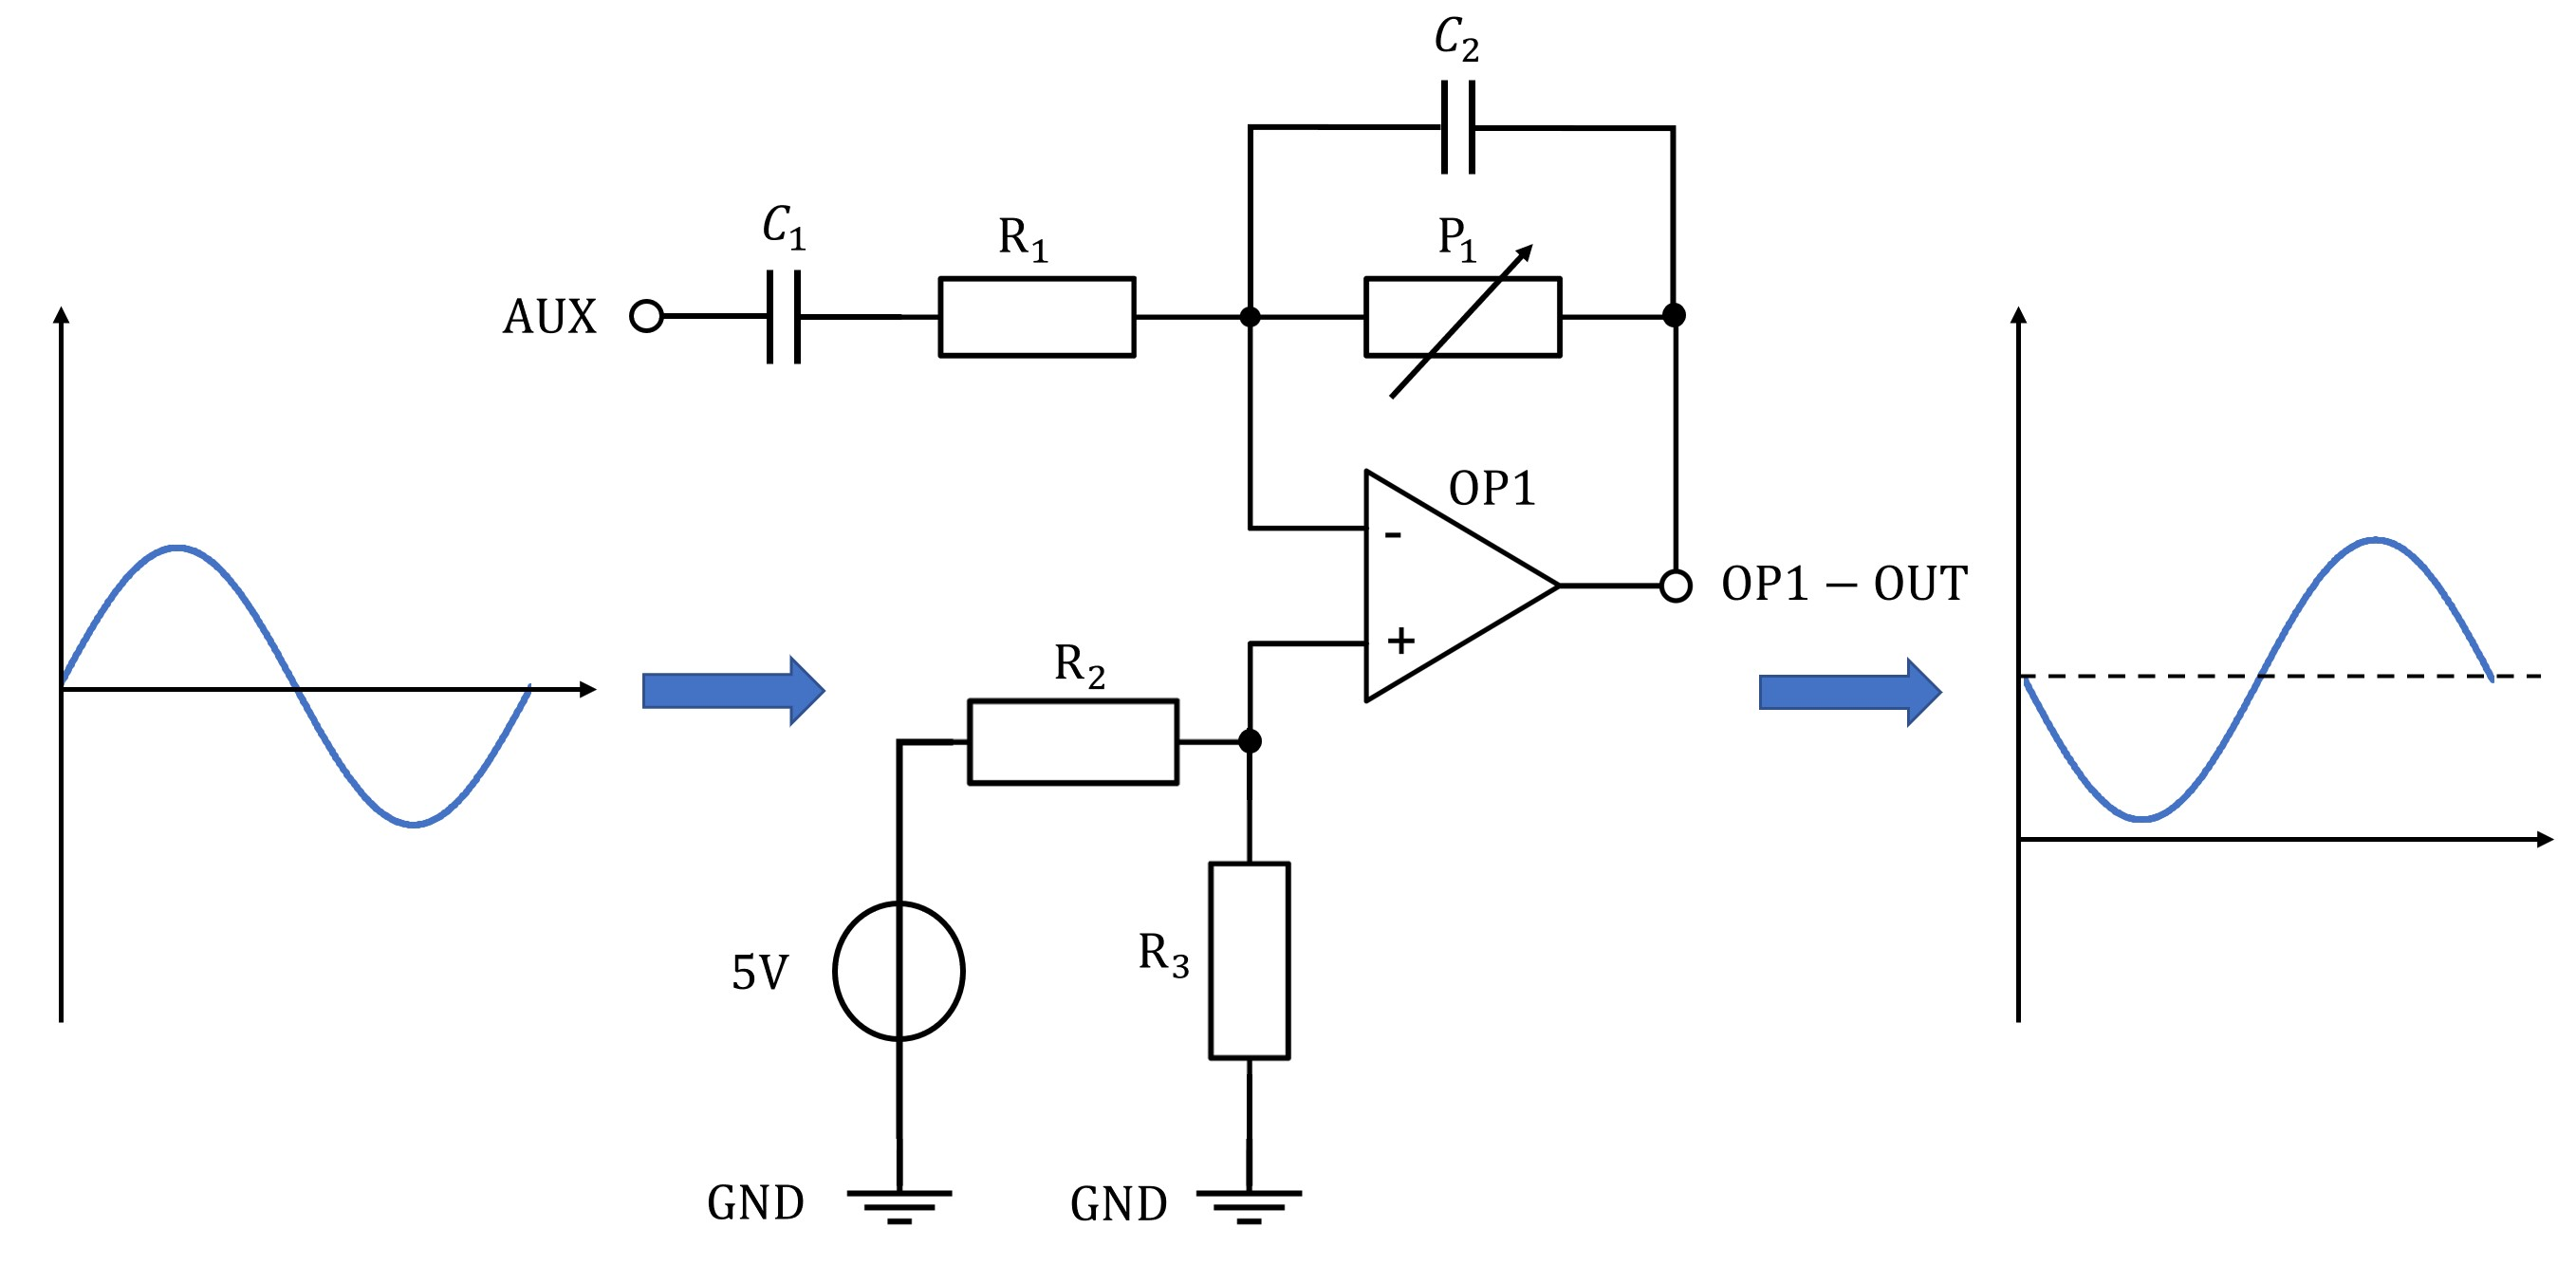
\includegraphics[width = 0.9 \textwidth ]{stufe1.jpg}
	\caption[Eingangssignalverarbeitungsstufe]{Eingangssignalverarbeitungsstufe} \gls{online:Eigen}
	\label{fig:stufe1}
\end{figure}

Der Schlüsselfaktor in der Eingangsstufe ist der variable Widerstand im Rückkopplungspfad des \gls{acr:OP}s. Hierbei handelt es sich um ein Digitales Potentiometer, welches sich über \gls{acr:SPI} vom Arduino zur Laufzeit beliebig verändern lässt. Die Schwierigkeit in der Implementierung dieses Bauteiles liegt jedoch darin, dass es keine negativen Spannungen verträgt. Aus dem Datenblatt ist ersichtlich, dass es nur mit Spannungen von $-0,6V<U<6V$ sorgfältig arbeiten kann. Da es sich bei dem zu verarbeitenden Audiosignal um ein Wechselstromsignal mit einer Amplitude von etwa 1,5V handelt, wurden in dieser Schaltung Vorkehrungen getroffen um die negativen Anteile dieses Signals in positive Anteile zu konvertieren. Um dieses Vorhaben zu realisieren wurde auf den nichtinvertierenden Eingang des \gls{acr:OP}s mithilfe eines Spannungsteilers $R_{3}$ und $R_{2}$ eine Spannung angelegt. Diese soll das Potential des \gls{acr:OP}s so anheben, dass das AC-Signal aus der Soundkarte direkt mit einem Offset addiert wird und somit keine negativen Anteile mehr besitzt. Um die Soundkarte vor der DC-Spannung zu schützen wurde ein DC Abblockkondensator $C_{1}$ am Signaleingang vorgesehen. Dieser ist für AC-Signale komplett durchlässig. Aufgrund der Annahme einer maximalen Amplitude von 1,5V muss also also ein Mindestoffset von 0,9V auf das Signal addiert werden. Um hier jedoch die Amplitude trotz Verstärkung innerhalb des erlaubten Spannungsbereiches von $-0,6V<U<6V$ bleiben wurde ein fester Offset von 2,15V gewählt. Zudem würde eine maximale Verstärkung von $A=2$ hinzugezogen wodurch sich der Spannungsbereich, selbst bei einer maximalen Verstärkung, stets in einem Bereich von $-0,2V<U<5,7V$ befindet. Dies ist in ~\ref{fig:ampoff} illustriert. 

\begin{figure}[H]
	\centering
	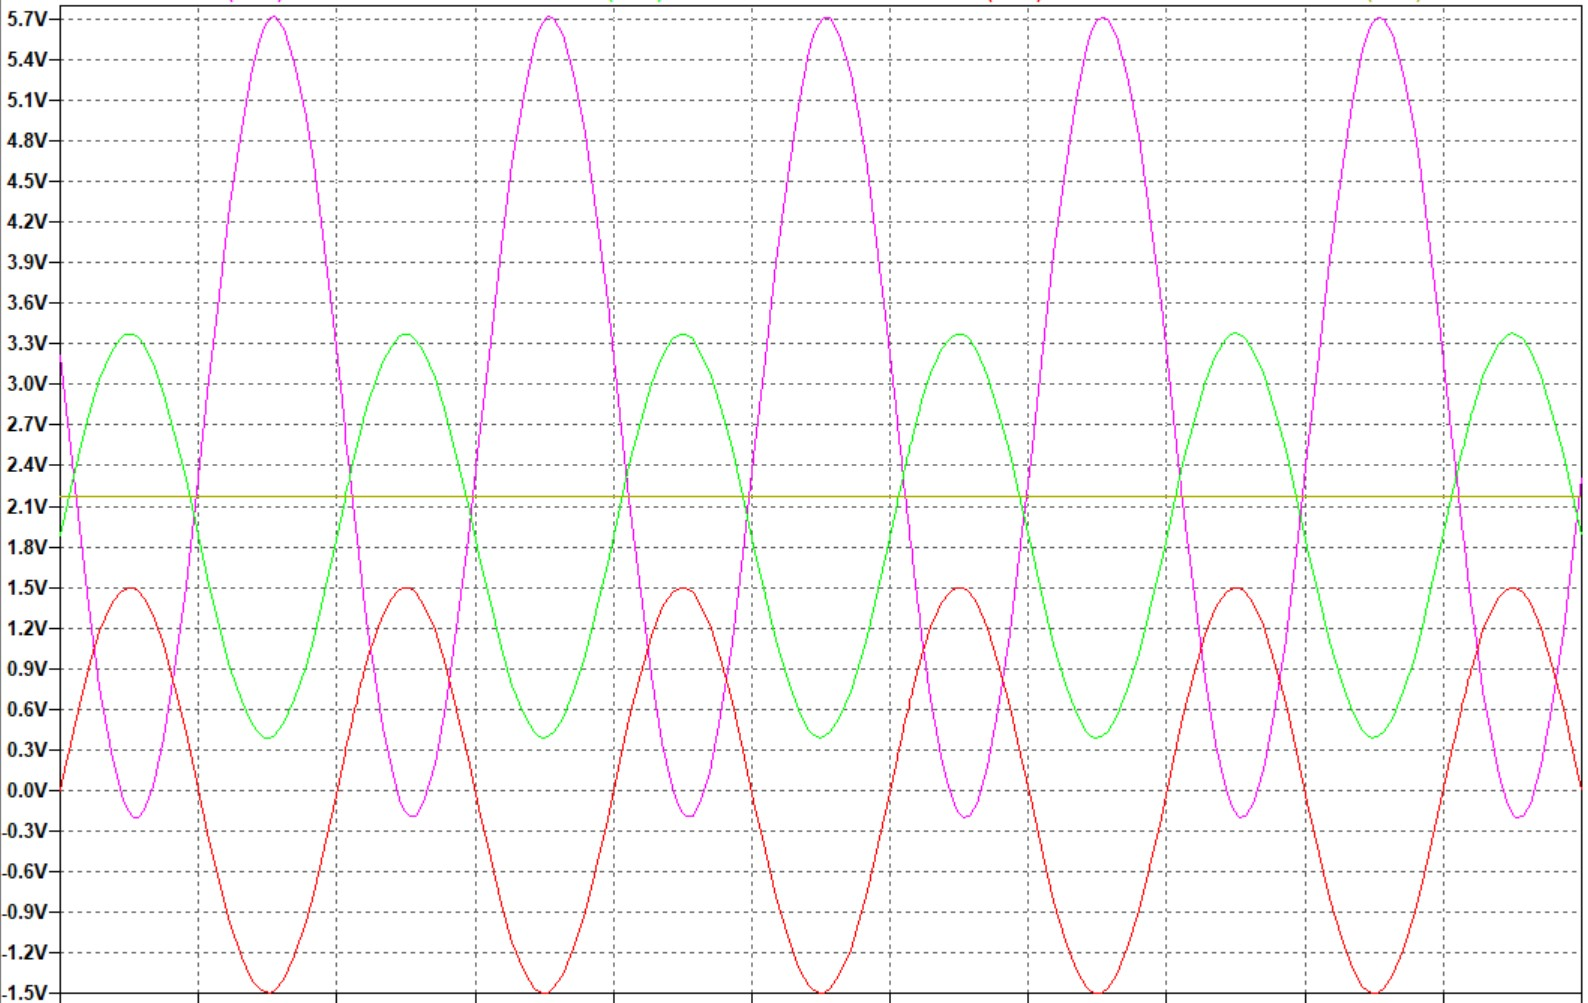
\includegraphics[width = 0.8 \textwidth ]{ampoff.jpg}
	\caption[Simulation von Offset und Verstärkung]{Simulation von Offset und Verstärkung} \gls{online:Eigen}
	\label{fig:ampoff}
\end{figure}

Somit kann gewährleistet werden, dass das Digitale Potentiometer zunehmend in einem legitimen Spannungsbereich betrieben wird.

Der zweite \gls{acr:OP} der Schaltung sorgt in der Signalkette für einen weiteren
Offset welcher die Grundhelligkeit der \gls{acr:LED} regelt. Da hier keine negative Spannung auftritt, kann das Digitale Potentiometer direkt angeschlossen werden.

\begin{figure}[H]
	\centering
	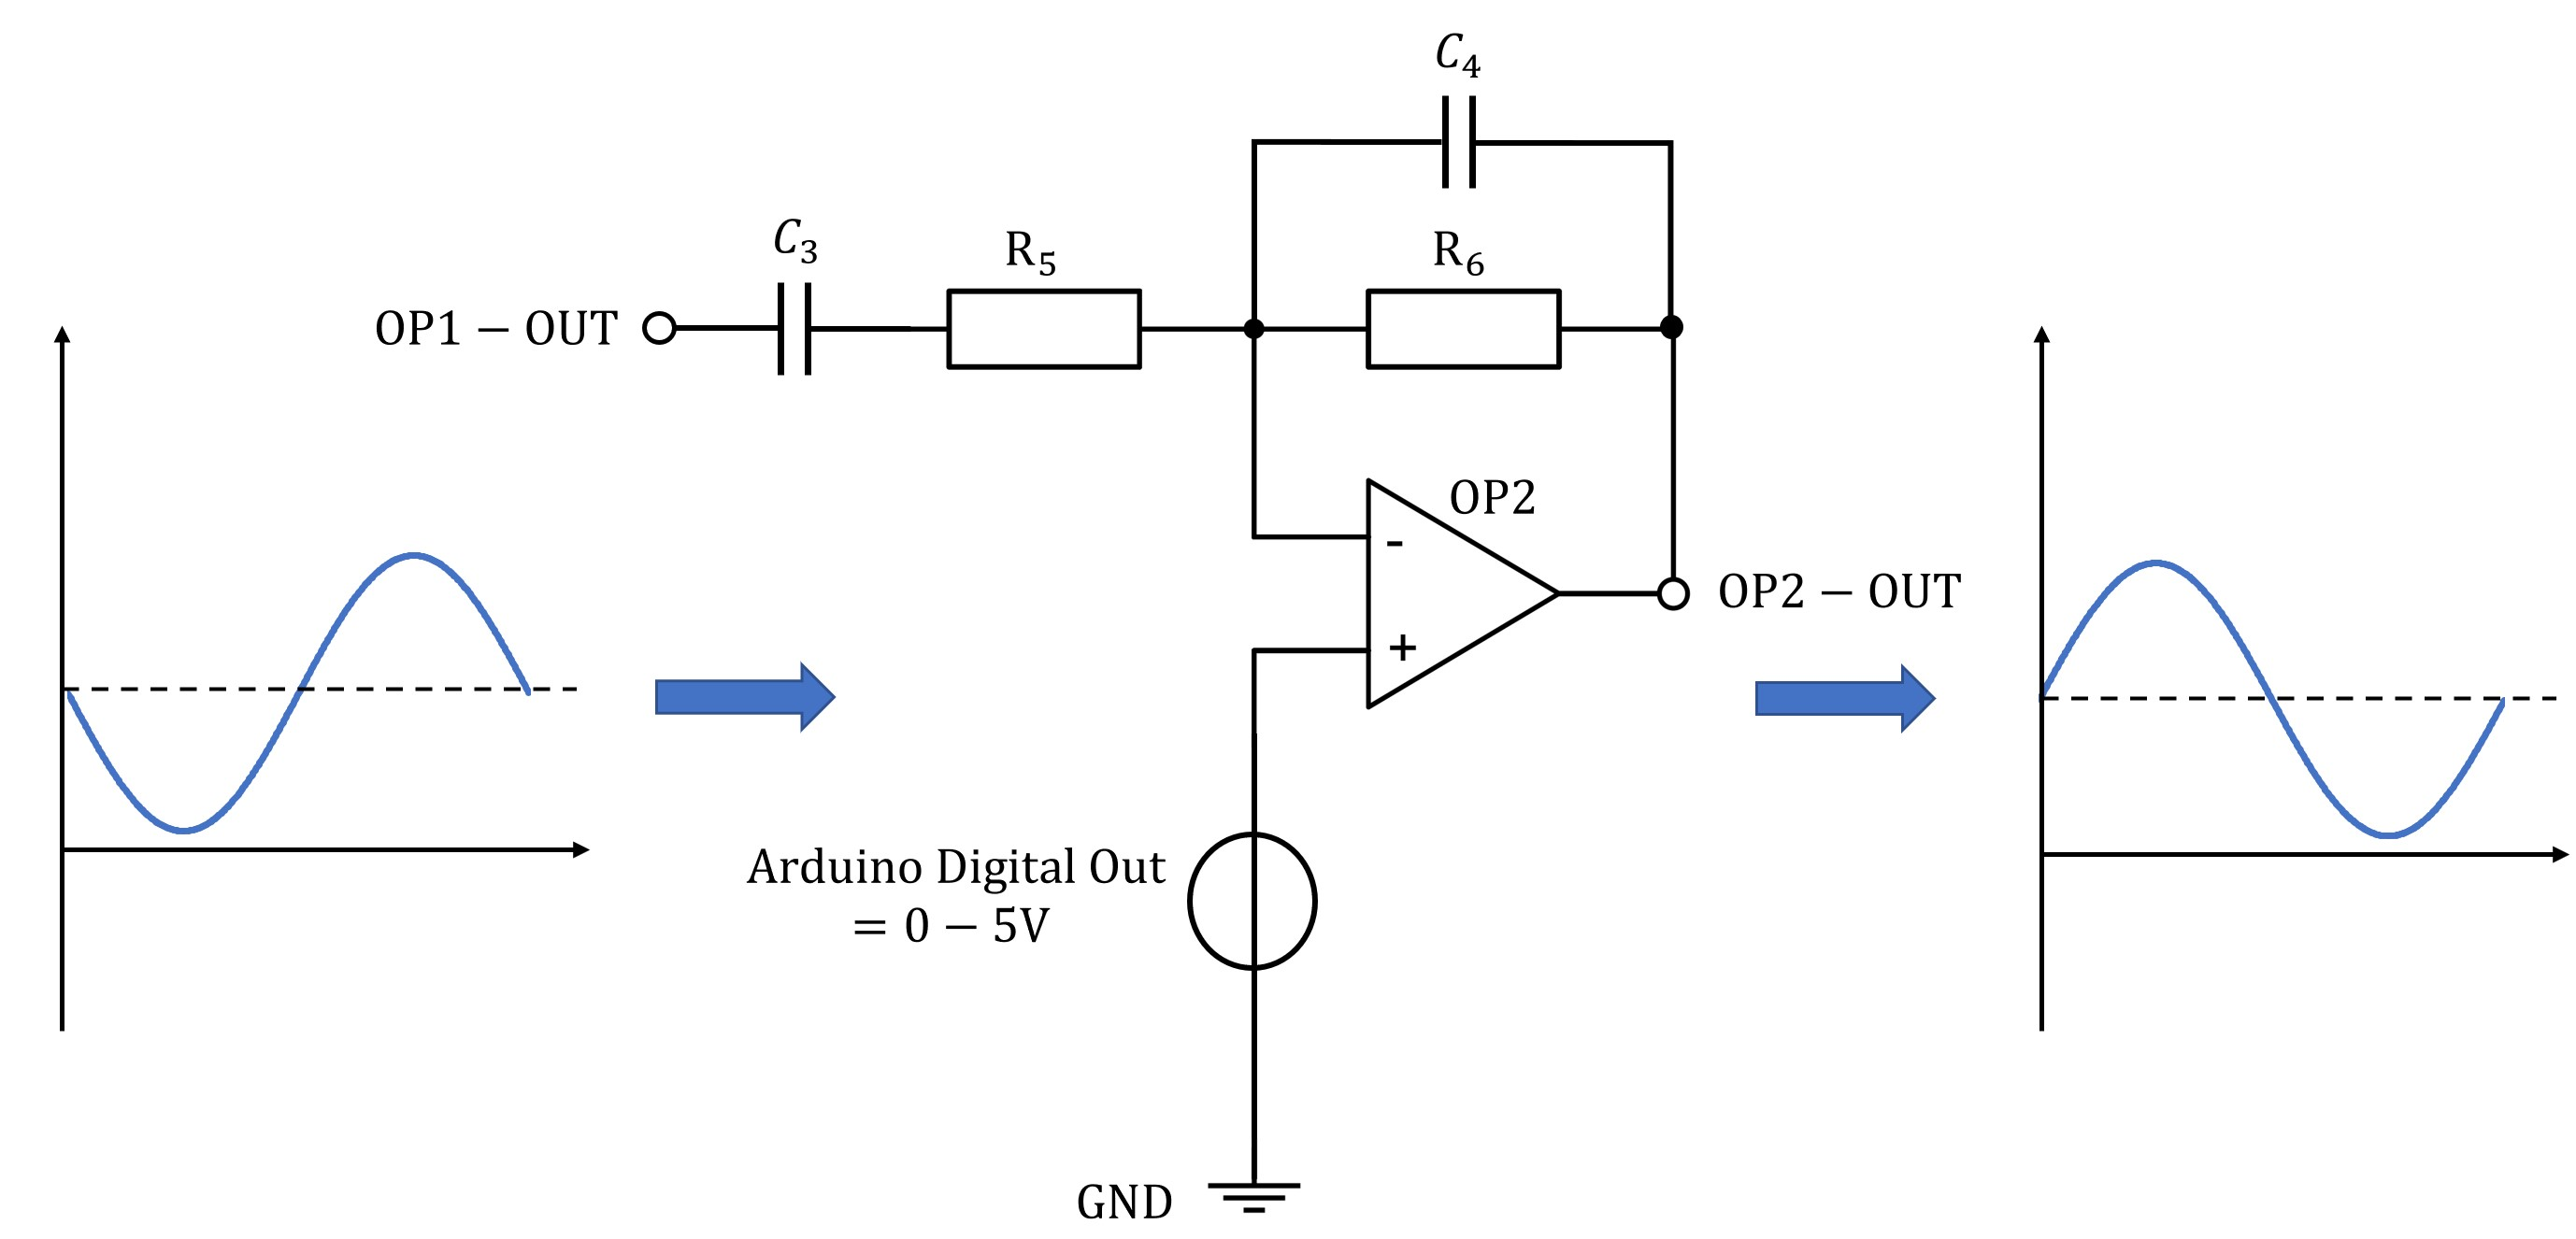
\includegraphics[width = 0.9 \textwidth ]{stufe2.jpg}
	\caption[Zweite Signalverarbeitungsstufe]{Zweite Signalverarbeitungsstufe} \gls{online:Eigen}
	\label{fig:stufe2}
\end{figure}


Die sehr hohe Vorwärtsverstärkung und die differentielle Eingangscharakteristik des \gls{acr:OP}s können genutzt werden, um eine nahezu ideale spannungsgesteuerte Stromquelle oder einen Spannungs-zu-Strom-Wandler zu realisieren. Es ist jedoch zu beachten, dass die umzuwandelnde Eingangsspannung an den nicht invertierenden Eingang des \gls{acr:OP}s angelegt wird. Der invertierende Eingang ist in Rückkopplung mit einem Ende des Widerstands $R{1}$ und der Source des Transistors $M{1}$ verbunden. Dies sorgt dafür, dass zwischen den Eingängen des \gls{acr:OP}s kein Spannungsunterschied herrscht. Der Ausgang des \gls{acr:OP}s steuert also das Gate des \gls{acr:MOSFET}s. Seine hohe Leerlaufverstärkung zwingt das Gate von $M{1}$ auf die erforderliche Spannung. Dadurch wird die Spannung, welche an $OP2-OUT = U_{R1}$ anliegt auf die Source des \gls{acr:MOSFET}s gespiegelt. Draus ergibt sich der Strom zu: 

\begin{equation}
	\label{equ:bsp1}
	I_{R1} = \frac{U_{R1}}{R_{1}}
\end{equation}

\begin{figure}[H]
	\centering
	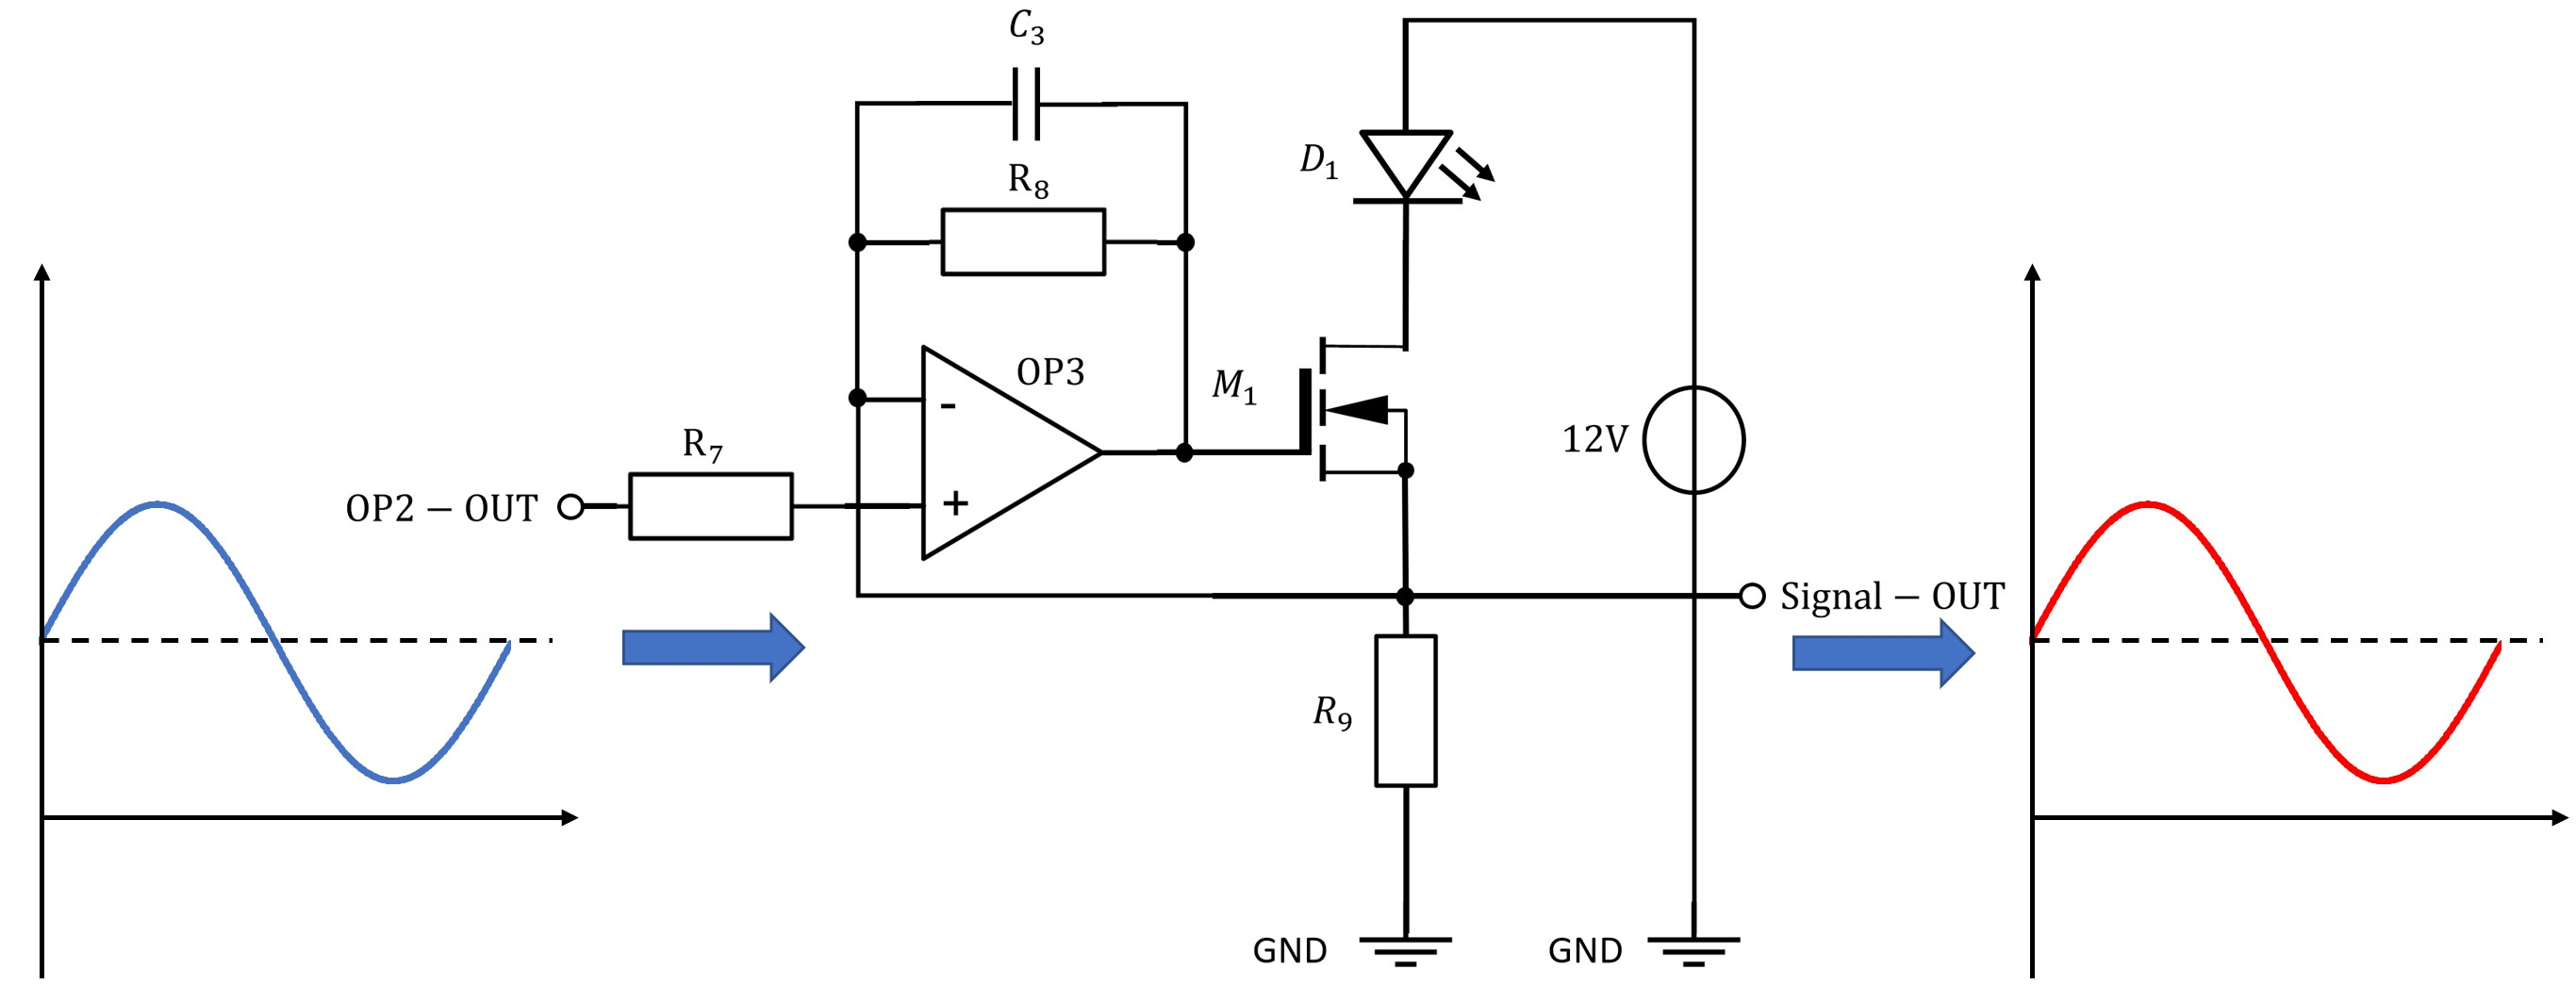
\includegraphics[width = 0.9 \textwidth ]{endstufe.jpg}
	\caption[LED- Treiber als Endstufe]{LED- Treiber als Endstufe} \gls{online:Eigen}
	\label{fig:endstufe}
\end{figure}

Durch die Bekanntheit des Stromflusses durch $R_1$ kann nun durch kirchhoffsche Regeln auf den Stromfluss in der \gls{acr:LED} geschlossen werden.\gls{online:vtoi} Dieser Strom wiederum erzeugt über selbigen Widerstand eine Anhebung des Potentials am - Eingang des \gls{acr:OP}s. Auf diese Weise versucht der \gls{acr:OP} seine beiden Eingänge auf das gleiche Potential anzuheben. Beim Leistungswiderstand $R_{9}$ handelt es sich um einen sehr kleinen Widerstand, weshalb durch die \gls{acr:LED}, den \gls{acr:MOSFET} und den Leistungswiderstand ein sehr hoher Strom fließt. Dieser sorgt für eine hell leuchtende \gls{acr:LED} zur Übertragung des Signals.

\subsection{Simulation in LT-Spice}
\label{subsec:Unterabschnitt1}

Das vorausgegangene theoretische Wissen wurde zudem mit einer LT-Spice Simulation überprüft. So konnten eventuelle Fehler bei der Dimensionierung ermittelt und verbessert werden werden. 

\begin{figure}[H]
	\centering
	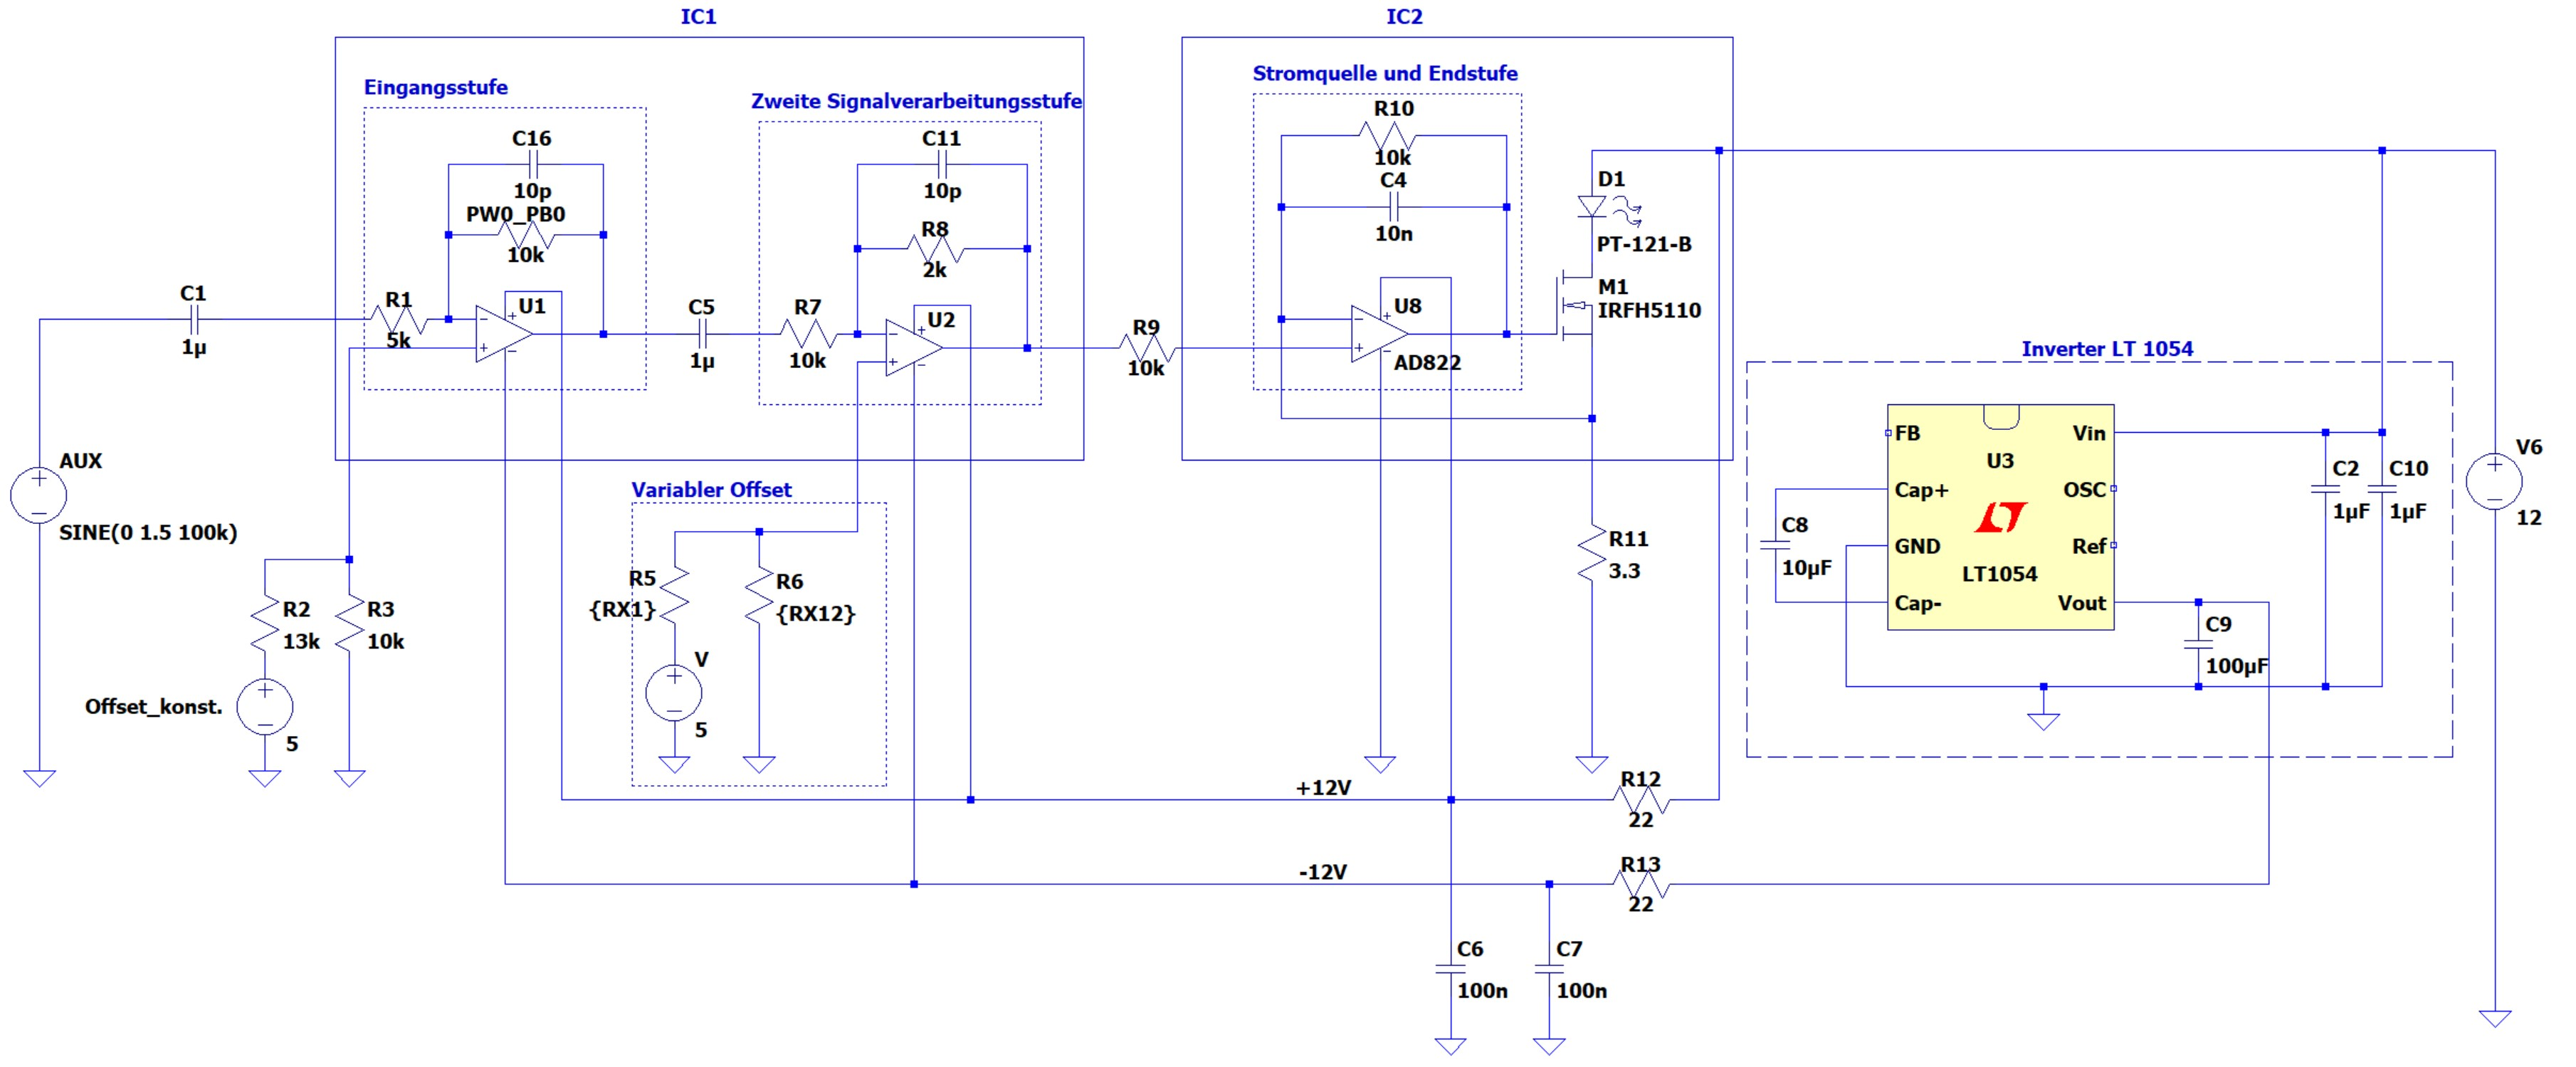
\includegraphics[width = 1 \textwidth ]{spice.jpg}
	\caption[LT-Spice Simulation der Signalverarbeitung]{LT-Spice Simulation der Signalverarbeitung} \gls{online:Eigen}
	\label{fig:spice}
\end{figure}

\subsection{Platinenlayout in Eagle}
\label{subsec:Unterabschnitt12}

Beim Platinenlayout Entwurf vom Senders wurde ein besonderes Augenmerk auf die Trennung von Signal und Leistungswegen geachtet.

\begin{figure}[H]
	\centering
	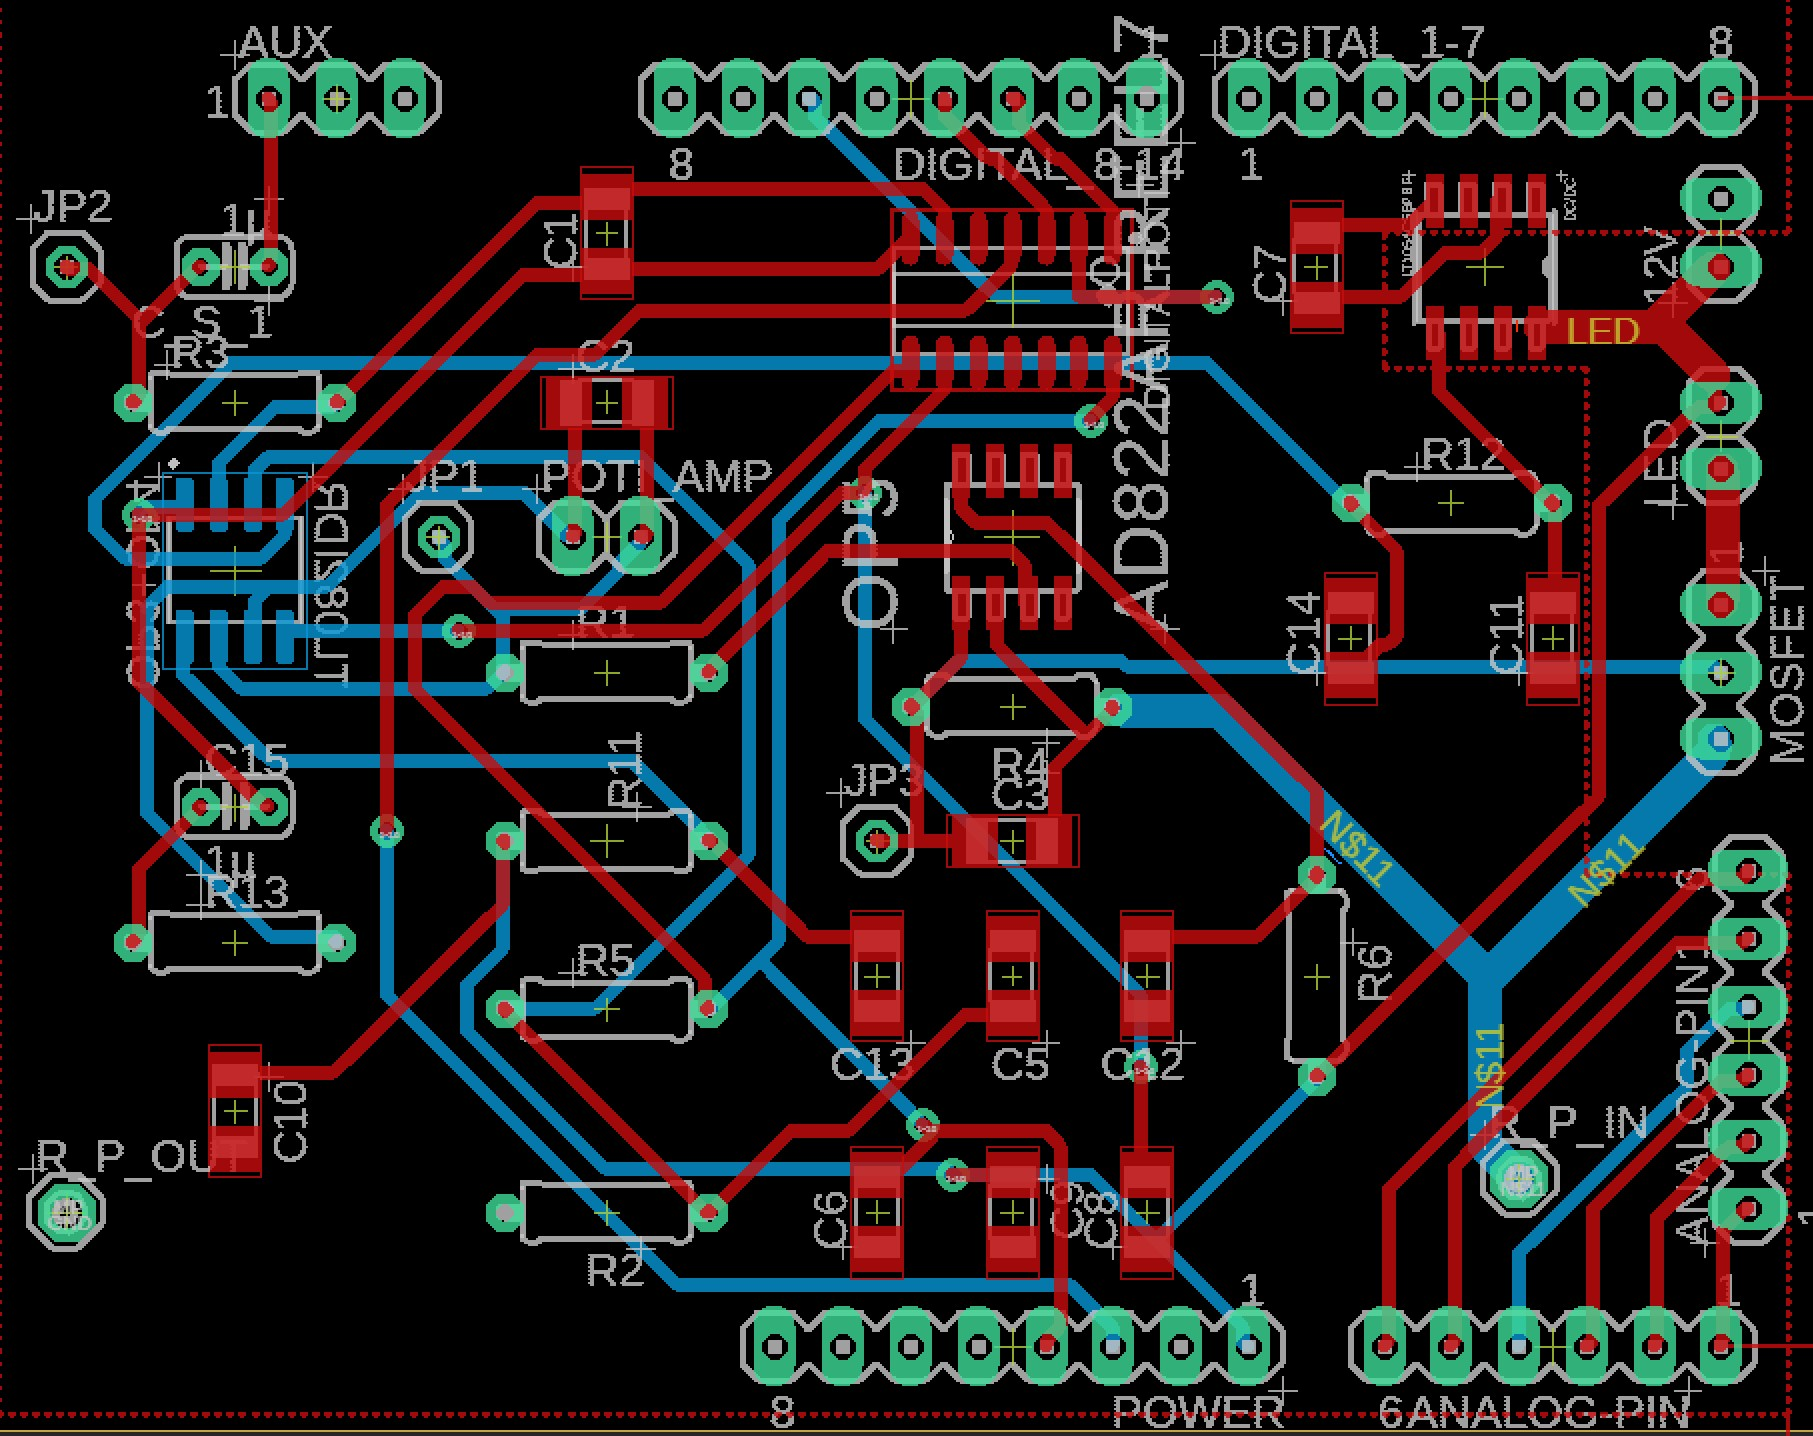
\includegraphics[width =0.8 \textwidth ]{eagle.jpg}
	\caption[Eagle Auszug der Platine]{Eagle Auszug der Platine} \gls{online:Eigen}
	\label{fig:eagle}
\end{figure}

Im unteren Bereich der Platine befindet sich der Leistungswiderstand, welcher sich von $R-P-IN$ zu $R-P-OUT$ erstreckt. Zuzüglich befinden sich der DC/DC Spannungswandler, \gls{acr:LED} und \gls{acr:MOSFET}, die signifikanten Bauteile der Stromquelle auf des Rechten Seite der Platine und somit möglichst weit vom Signalverarbeitungspfad entfernt. In der Schaltung fließen teilweise Ströme bis 1,35A. Da es bei solch hohen Strömen zu Problemen mit der   \gls{acr:EMV} kommen kann, wurde der Signalweg linksseitig auf der Platine positioniert. Außerdem wurden die Leiterbahnen im Leistungspfad besonders breit ausgelegt, da hier große Ströme fließen. Genaue Informationen über die Dimensionierung der Leiterbahnen und Abstände ist in Tabelle~\ref{tab:leiterbahnen} zu finden. Auf der Platine wurden für die Operationsverstärker, das Digitalpotentiometer und den DC/DC Spannungswandler IC-Sockel aufgelötet. Das ermöglicht den schnellen Austausch von defekten Bauteilen. Die komplette Schaltung des \gls{acr:VLC}-Senders wurde auf die Größe einer kleinen gefrästen Platine untergebracht. Deshalb wurden Leitungen auf der Rückseite der Platine verlegt. Diese sind in Abbildung ~\ref{fig:eagle} durch die Blauen Leiterbahnen dargestellt. Des weiteren wurden im Signalverarbeitungspfad nach jeder Stufe Pins vorgesehen, um die Fehlersuche zu erleichtern und nachträglich einzelne Funktionsprüfungen durchzuführen. Hinzu ist zu beachten, dass die Bauteile im Leistungspfad durch den hohen Stromfluss eine hohe thermische Abgabe an Energie verzeichnen müssen. Um diese zu reduzieren wurden Kühlkörper vorgesehen. Wie diese Berechnet und Dimensioniert werden wird in Kapitel ~\ref{subsub:thermo} näher erläutert. Um die Schaltung zuletzt noch zusätzlich weniger Störanfällig zu gestalten, wurden die gegebenen freien Flächen auf beiden Seiten der Platine mit dem Masse Potential ausgefüllt. 

\subsection{Thermisches Management}
\label{subsub:thermo}
Wie im vorherigen Kapitel schon erwähnt, fließt durch den Leistungsstrang der Schaltung ein sehr hoher Strom. Durch diesen hohen Stromfluss kommt es zu einer immensen Hitzeentwicklung in den Bauteilen. Um jedoch die einwandfreie Funktion von elektronischen Halbleiterbauelementen zu gewährleisten, ist die Einhaltung der vom Hersteller angegebenen maximalen Sperrschichttemperaturen unerlässlich. Solch eine Sperrschichttemperatur lässt sich nur bei geringer Leistungsanforderung ohne Kühlung einhalten. Zudem sind die Einbaulage, der Einbauort, die Geschwindigkeit und Temperatur der Umgebungsluft variable Größen die miteinzukalkulieren sind.\gls{online:thermo}

\begin{figure}[H]
	\centering
	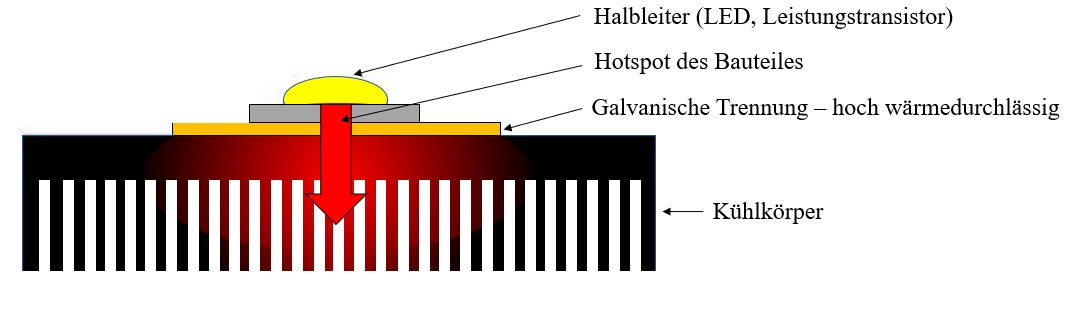
\includegraphics[width =1 \textwidth ]{thermo.jpg}
	\caption[Montageschema eines Kühlkörpers]{Montageschema eines Kühlkörpers} \gls{online:Eigen}\gls{online:thermo2}
	\label{fig:thermo}
\end{figure}

Um gegen diese Hitzeentwicklung vorzugehen wird für die kritischen Bauteile somit ein Kühlkörper vorgesehen. Diese sollen die Wärme vom Bauteil weg und nach außen hin abführen. In dem hier gegebenen elektrischen Stromkreis, werden zwei Halbleiter als kritische und zu kühlende Bauteile betrachtet. Zunächst die \gls{acr:LED} zum Übertragen des Signals und zum zweiten der \gls{acr:MOSFET}.\cite{thermLED}

Zur Auswahl eines geeigneten Kühlkörpers für ein Halbleiterbauelement ist die Berechnung des Wärmewiderstandes unerlässlich. Dafür werden die in Tabelle~\ref{tab:thermofaktoren} aufgeführten Variablen in folgende Gleichung eingesetzt.

\begin{equation}
	\label{equ:thermo}
	R_{thK} = \frac{\vartheta_{i}-\vartheta_{u}}{P}-(R_{thG}+R_{RthM})
\end{equation}

\begin{table}[htb]
	\begin{center}
		\begin{tabular}[h]{cl}	
			\toprule
			Faktor & Bedeutung \\
			\midrule
			$\vartheta_{i}$& Herstellerangabe der Halbleiters zur max. Sperrschichttemperatur\\
			$\vartheta_{u}$& Umgebungstemperatur in $^\circ C$ \\
			$P$ &  Die am zu kühlenden Halbleiter maximal anfallende Leistung in Watt\\
			Rth & Wärmewiderstand allgemein in $\frac{K}{W}$ \\
			RthG & Herstellerangabe zum innerer Wärmewiderstand des Halbleiters \\
			RthM & Wärmewiderstand der Montagefläche \\
			RthK &  Wärmewiderstand des Kühlkörpers \\
			\bottomrule
		\end{tabular}
		\caption{Variablen zu berechnung des Kühlkörpers}\gls{online:thermo1}
		\label{tab:thermofaktoren}
	\end{center}
\end{table}

Für die Berechnung der Kühlkörper wurden zudem Berechnungen zur Verlustleistung des
\gls{acr:MOSFET}s und der \gls{acr:LED} vorgenommen. Es wird bewusst überdimensioniert. Dazu wurde beispielsweise für die \gls{acr:LED} mit einem Wirkungsgrad von 0 \% gerechnet. Unter diesen Umständen würde die Verlustleistung 100 \% betragen. \gls{acr:LED}s haben jedoch tatsächlich einen Wirkungsgrad von ca. 25 - 50 \%. Die maximalen Verluste werden natürlich bei voller Helligkeit verzeichnet. Zur Auslegung der Kühlkörper wurden also folgende Berechnungen durchgeführt:

\begin{equation}
	\label{equ:thermoled}
	P_{LED} = U_{LED} \cdot I_{G} = 3,12V \cdot 1,42A= 4,43W
\end{equation}

\begin{equation}
	\label{equ:thermomos}
	P_{MOSFET} = U_{MOSFET} \cdot I_{G} = 4,1V \cdot 1,42A= 5,86W
\end{equation}

Wodurch sich der Wärmewiderstand der Kühlkörper für die \gls{acr:LED} zu

\begin{equation}
	\label{equ:thermo2}
	R_{thK-LED} = \frac{35 ^\circ C - 25 ^\circ C}{4,43W}-(1 \frac{^\circ C}{W}+0,1 \frac{^\circ C}{W}) = 1,36\frac{^\circ C}{W}
\end{equation}

berechnet und der Wärmewiderstand des \gls{acr:MOSFET} aus
 
\begin{equation}
	\label{equ:thermo3}
	R_{thK-MOSFET} = \frac{50 ^\circ C - 25 ^\circ C}{5,86W}-(1,15 \frac{^\circ C}{W}+0,1 \frac{^\circ C}{W}) = 3,22\frac{^\circ C}{W}
\end{equation}

ergibt. Gewählt wurde zuletzt für sowohl \gls{acr:LED} als auch \gls{acr:MOSFET} ein Kühlkörper in der Größenordnung von 3 $^\circ C/W$.

\subsection{Planung und Aufbau des Gehäuses}
\label{subsec:geh}

In den vorausgegangenen Unterkapiteln wurden sowohl die Schaltungsteile, als auch die Wichtigkeit einer ausreichenden Kühlung der Bauteile verdeutlicht. Nun galt es all diese Hardwarekomponenten zu einem großen ganzen zusammen zu fassen um somit ein in sich beständiges System zu schaffen. Demnach wurde für die kompakte und ansehnliche Unterbringung aller Hardwarekomponenten ein 3D-Druck-Gehäuse projektiert. Hierbei wurde so platzsparend wie möglich gearbeitet. Aussparungen für die Datenschnittstelle und Spannungsversorgung wurden so angeordnet, dass diese jederzeit zugänglich sind. Zudem wurden drei Seiten mit ausreichend Lüftungsschlitzen bestückt, um der Wärmeentwicklung im Gehäuse entgegen zu wirken. Um diese thermische Entwicklung noch weiter unter Kontrolle zu bringen wurde eine Aussparung für einen mit $12V$ betriebenen Lüfter vorgesehen. Dieser soll den Luftstrom im Gehäuse anregen um somit eine bessere Kühlung zu gewährleisten. Abbildung~\ref{fig:3dbottom} veranschaulicht die 3D-Ansicht dieses Gehäuses.

\begin{figure}[H]
	\centering
	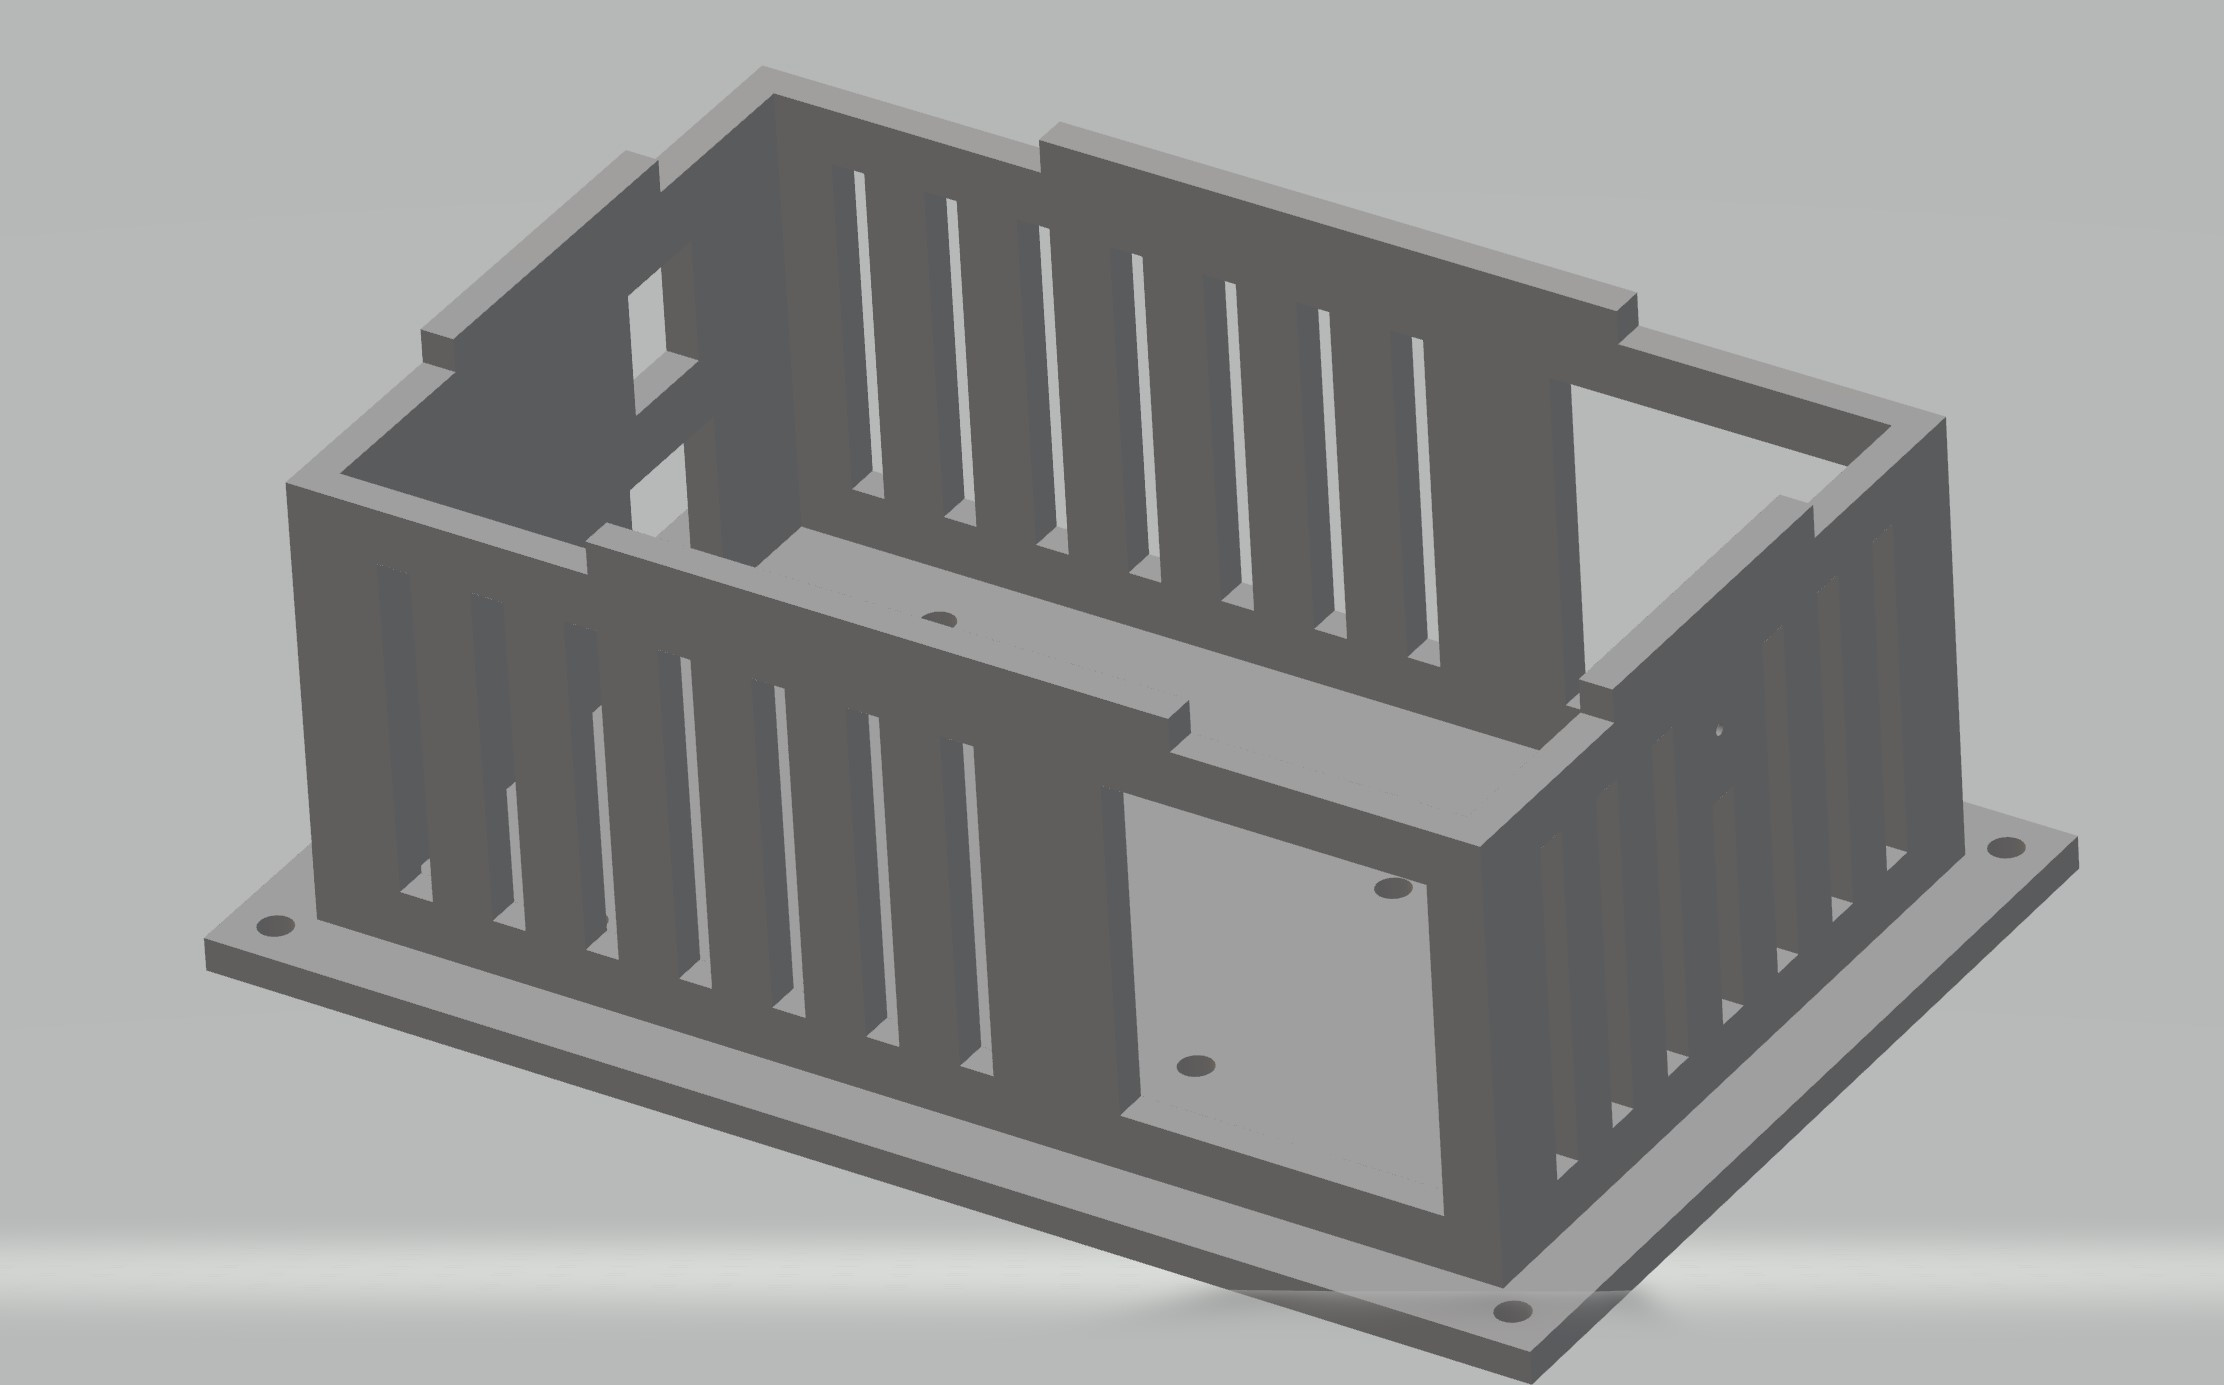
\includegraphics[width =1 \textwidth ]{3dbottom.jpg}
	\caption[Boden des 3D-Drucks]{Boden des 3D-Drucks} \gls{online:Eigen}
	\label{fig:3dbottom}
\end{figure}

Der Arduino wird am Boden des Gehäuses fixiert und bietet die Basis des Analogen Schaltungsteils.
Da sich Leistungswiderstand, Transistor und Leuchtdiode im Betrieb stark erhitzen, wurden die zugehörigen Kühlkörper nah am Lüfter montiert. Zusätzlich wurde im Deckel eine Öffnung für den Einbau eines LCD-Displays vorgesehen um dort Daten visuell am Sender auszugeben. Für die Datenübertragung wurde eine \gls{acr:AUX}-Buchse in der Nähe der Spannungsversorgung verbaut.

\begin{figure}[H]
	\centering
	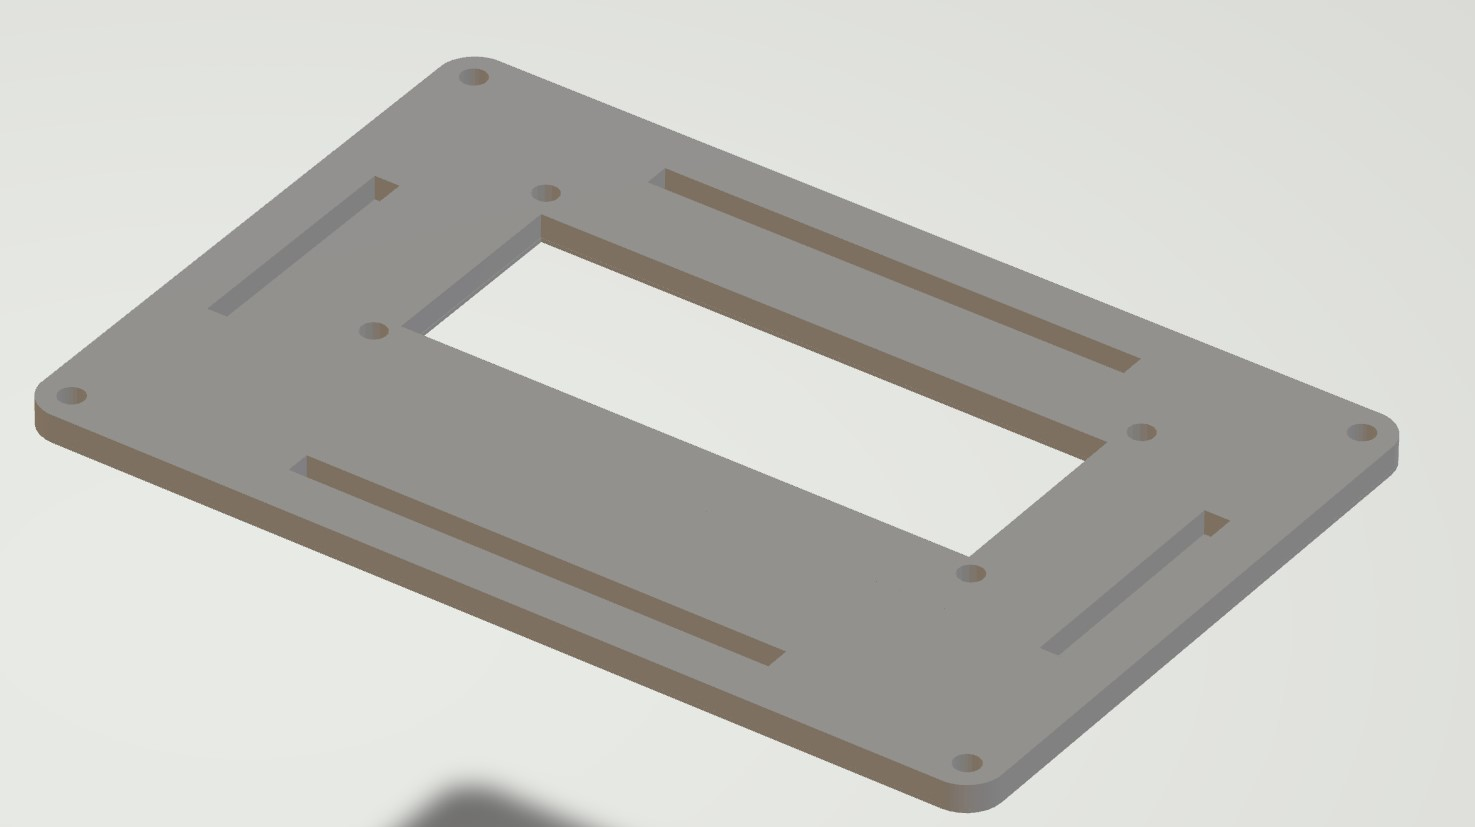
\includegraphics[width =1 \textwidth ]{3dtop.jpg}
	\caption[Boden des 3D-Drucks]{Boden des 3D-Drucks} \gls{online:Eigen}
	\label{fig:3dtop}
\end{figure}
\newpage
\section{Software}
\label{sec:Software}

Dieser Abschnitt beschäftigt sich mit der, in der Arduino \gls{acr:IDE} programmierten, Ansteuerung des Zwei-Kanal Digitalpotentiometers zur Variation des Offsets und der Amplitude. Dabei soll das prinzipielle Funktionsschema und dessen Implementierung zum Ausdruck gebracht werden. Im Anschluss wird die Konfigurierung und Evaluierung der Übertragung via Dream Software näher beschrieben und charakterisiert.

\subsection{Offset-Regelung}
\label{subsec:offset}
Um ein Potentiometer mit dem Arduino einlesen zu können, muss einer der analogen Eingabepins des Arduino verwenden. Da Potentiometer drei Anschlüsse besitzen, schließt man einen der äußeren Kontakte des Schleifenwiderstands an der 5V Spannungsquelle an und den anderen auf Ground. Den mittleren Anschluss, welcher für die Variabilität des Potentiometer steht, wird mit dem analogen Eingang A0 des Arduino verbunden. Abbildung~\ref{fig:digipot} illustriert dies. 

\begin{figure}[H]
	\centering
	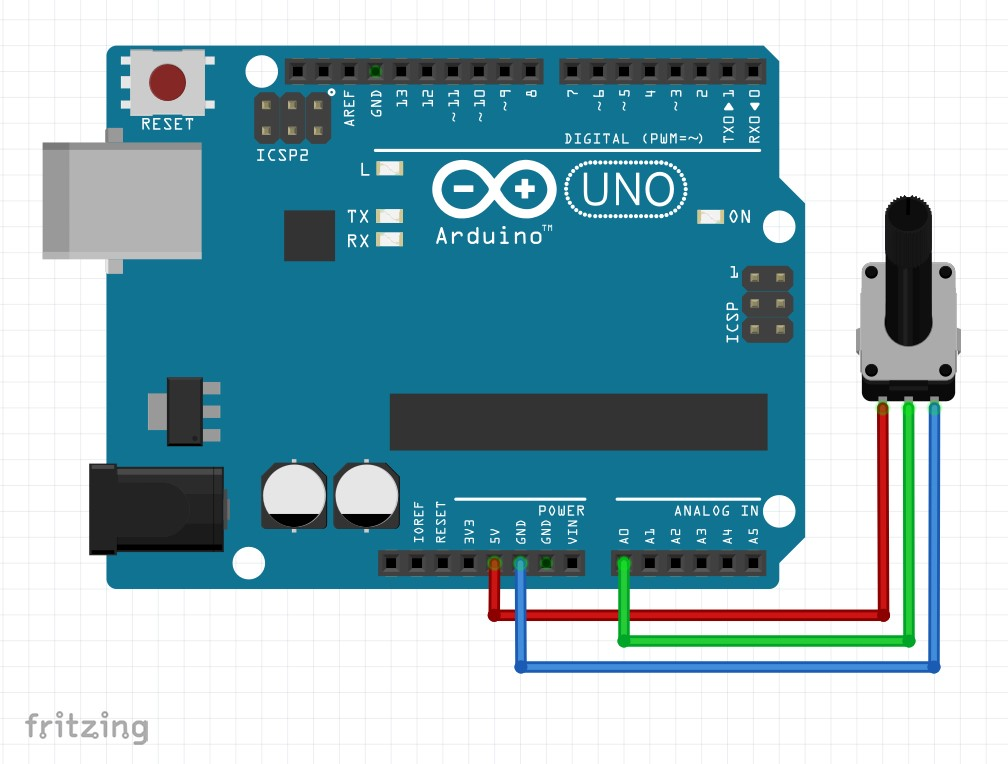
\includegraphics[width =0.8 \textwidth ]{digipot.jpg}
	\caption[Anschlussschema des Potentiometer]{Anschlussschema des Potentiometer} 
	\gls{online:Eigen}\gls{online:fritz}
	\label{fig:digipot}
\end{figure}

Der analoge Pin $A0$ wird in der Arduino \gls{acr:IDE} durch die Funktion analogRead eingelesen. Die Arduino-Boards beherbergen einen 10-Bit-Analog-zu-Digital-Konverter. Dies hat zur folge, dass das Board Eingangsspannungen zwischen 0 und 5 V auf Integer-Werte zwischen 0 und 1023 mappt. Die erreichte Auflösung ist damit auf dem gegebenen Arduino UNO, 4,9 mV per Bit.\gls{online:analogread} Diese 1023 gilt es dann durch vier zu teilen, da ein Digital Potentiometer nur in 256 Stufen angesteuert werden kann. Der Wert wird dann über die \gls{acr:SPI} Schnittstelle an das Digital Potentiometer gesendet und verändert somit dessen Widerstandswert. Somit kann der Offsetwert extern in das Programm geschrieben werden. Dies ist so bedeutsam, da der Offset auch in der Amplituden-Regelung eine entscheidende Aufgabe hat. 

\subsection{Automatisierte Amplituden-Regelung}
\label{subsec:autoamp}
In Abbildung 16 wird die zur Steuerung Grundlegende Funktion des Programms erklärt, der zugehörige Quellcode kann im Kapitel Programmcode nachgelesen werden. Nach Initialisierung der Helligkeit der Lampe durch den Benutzer (Zwischen 0 und 255) wird aufgrund des gewählten Bereichs eine von zwei Berechnungen für die Amplitude vorgenommen. Dies kommt von der Begrenzung der Amplitude nach oben und
unten durch die LED. Falls sich der Offset, was hier für die Helligkeit steht, nun in der Mitte
befindet, kann die Amplitude des Signals Maximal werden. Weil durch diese Einordnung Werte zwischen 0 und 127 erreichen kann, wird der Wert der Amplitude noch mit einem Faktor von 2 Multipliziert. Der Zusammenhang zwischen Digitalwert und Verstärkung  kann in Kapitel Berechnung der Amplitudenverstärkung nachgelesen werden.

Durch den möglichen Widerstandsbereich des Digitalpotentiometers von 52 bis 10k lässt sich ein Spannungsteiler für die Spannungsquelle zur Einstellung des Amplituden Offsets mithilfe des OPs realisieren. Die Berechnung dafür zeigt Abbildung 17.

Berechnung der Amplitudenverstärkung
Wie in Kapitel Digital Potentiometer MCP42010 und Kapitel Berechnung des Amplitudenoffset beschrieben, lässt sich durch den Digitalpotentiometer ein absoluter Widerstandsbereich von 52 bis 10k einstellen. Für die Amplitudenverstärkung des Signals wird der Widerstand zwischen Schleiferkontakt RW0 und Kontakt RB0 abgegriffen. Dieser berechnet sich wie in Abbildung 19 gezeigt. Quelle: Datenblatt Abbildung 19: Berechnung des Widerstandsverhältnis. Damit kann ein Rückkopplungswiderstand von 52 bis 10 k erreicht werden. Die Verstärkung eines Invertierenden Verstärkers berechnet sich lt. Gleichung 1 mit dem vorgesehenen 10 k Vorwiderstand zu Verstärkungsfaktoren von

\subsection{Modulation mit Dream}
\label{subsec:dream}
Nun sollen Audio Echtzeitdaten in \gls{acr:DRM}-Format moduliert und über die aufgebaute Hardware versendet werden. Deshalb wird im folgenden erläutert wie die Dream Software zu verwenden ist. Sie verfügt über zwei verschiedene Möglichkeiten aufgerufen werden. Zum ersten im Sendemodus und zum zweiten im Empfangsmodus, wodurch bei einer Übertragung die Benutzung von zwei verschiedenen Computern vorausgesetzt wird. Zudem bietet Dream umfangreiche Einstellungsoptionen um sowohl Rauschen als auch andere Störungen zu minimieren. Die wichtigsten Parameter für die korrekte Benutzung und potentielle Fehlersuche werden in den folgenden zwei Kapiteln näher erläutert.


\subsubsection{Dream Transmitter}
\label{subsubsec:dreamtx}
Zum Start der Software ”Dream” im Übertragungsmodus muss das Programm mit dem parameter ”- t” gestartet werden. Die einfachste Möglichkeit für einen Programmstart mit Parameter bietet eine Verknüpfung, welche wie in Abbildung 15 gezeigt, angepasst wird. Das Zielverzeichnis darf dabei nicht verändert werden! Dieser Schritt muss nur einmal gemacht werden und man kann jederzeit den Übertragungsmodus starten indem man die Dream software über diese geänderte Verknüpfung startet.

\begin{figure}[H]
	\centering
	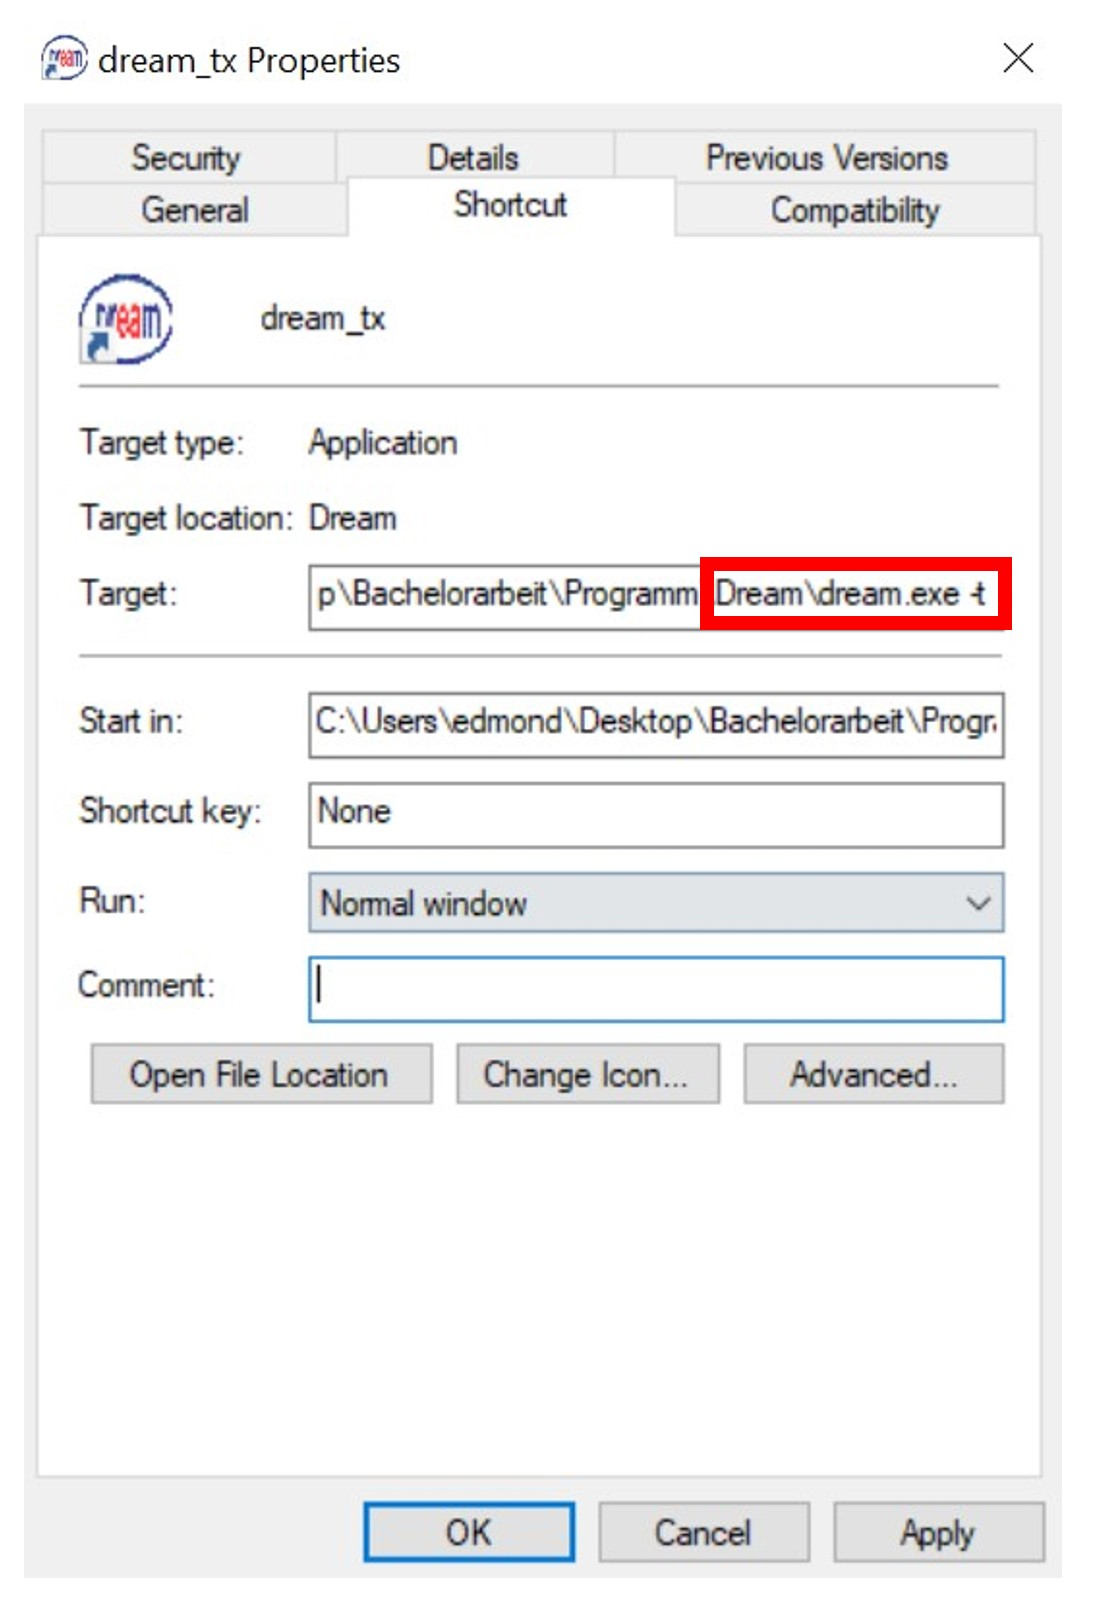
\includegraphics[width = 0.5 \textwidth ]{dreamtx.jpg}
	\caption[Modifizierung für den Sendemodus]{Modifizierung für den Sendemodus} \gls{online:Eigen}
	\label{fig:dreamtx}
\end{figure}

\begin{figure}[H]
	\centering
	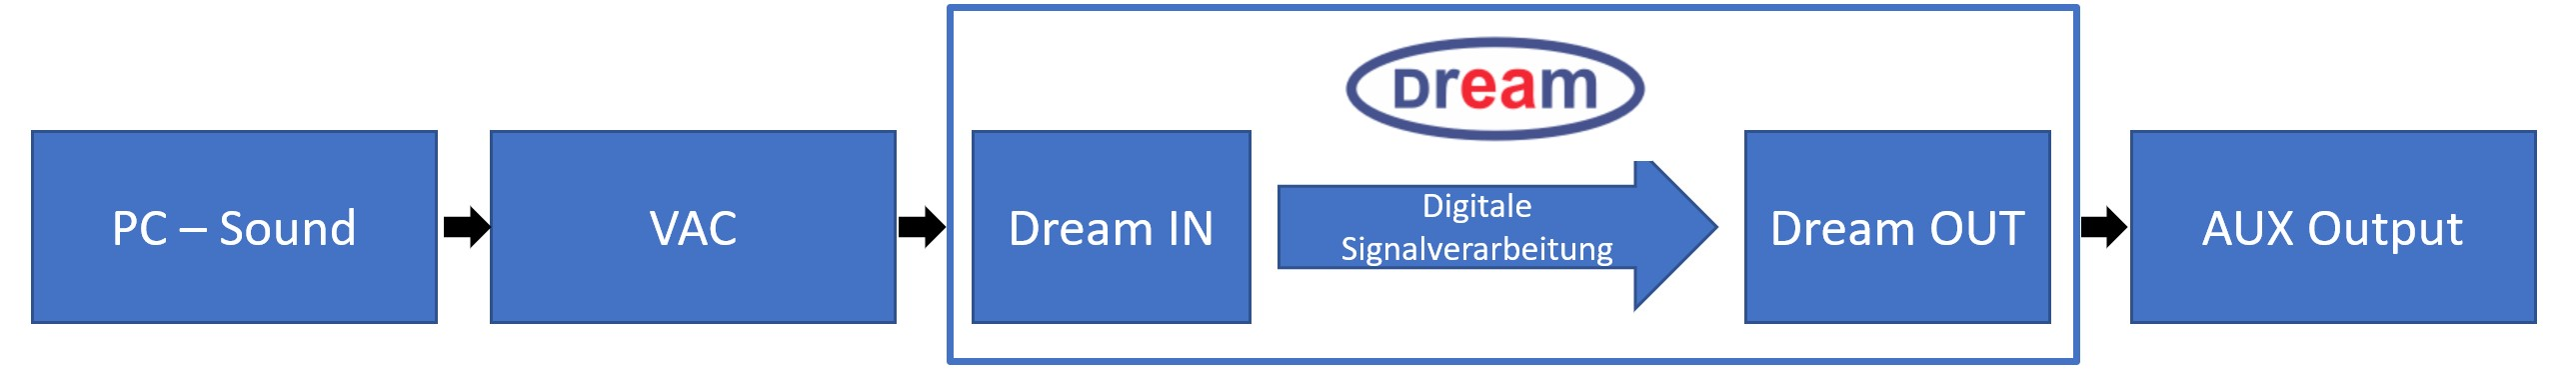
\includegraphics[width = 0.9 \textwidth ]{dreamtxeinstellung.jpg}
	\caption[Internes Audiorouting]{Internes Audiorouting} \gls{online:Eigen}
	\label{fig:dreamtxeinstellung}
\end{figure}

\begin{table}[h]
	\begin{center}
		\begin{tabular}{|p{0.28\linewidth} | p{0.72\linewidth}|}	
			\toprule
			\textbf{Parameters} &\textbf{Beschreibung}\\
			\midrule
			\textbf{\gls{acr:DRM} mode/ bandwidth} & In einem \gls{acr:DRM}-System sind vier mögliche Robustheitsmodi definiert, um das System an unterschiedliche Kanalbedingungen anzupassen.:\newline
			\textbf{Mode A}: Gaußsche Kanäle, mit geringem Fading.\newline
			\textbf{Mode B}: Zeit- und frequenzselektive Kanäle, mit längerer Verzögerungsspanne.\newline
			\textbf{Mode C}: Wie Robustheitsmodus B, jedoch mit höherer Dopplerspreizung.\newline
			\textbf{Mode D}: Wie Robustheitsmodus B, jedoch mit starker Verzögerung und Dopplerspreizung.\newline
			Die Bandbreite ist die Bruttobandbreite des aktuellen \gls{acr:DRM}-Signals. \\
			\midrule
			\textbf{Interleaver Depth} & Die Symbol-Interleavertiefe kann entweder kurz (ca. 400 ms) oder lang (ca. 2 s) sein. Je länger der Interleaver, desto besser kann der Kanaldecoder Fehler aus langsam schwindenden Signalen korrigieren. Aber je länger die Interleaver-Länge, desto länger die Verzögerung, bis Audio zu hören ist.\\
			\midrule			
			\textbf{\gls{acr:SDC} / \gls{acr:MSC}} & Zeigt die Modulationsart des \gls{acr:SDC}- und \gls{acr:SDC}-Kanals an. Für den \gls{acr:MSC}-Kanal sind einige hierarchische Modi definiert, die einen sehr stark geschützten Dienstkanal bieten können.\\
			\midrule
			\textbf{Prot. Level (B/A)} & Die Fehlerschutzstufe des Kanalcodierers. Für 64-QAM gibt es vier Schutzstufen, die im DRM-Standard definiert sind. Schutzstufe 0 hat den höchsten Schutz, während Stufe 3 den niedrigsten Schutz hat. Die Buchstaben A und B sind die Bezeichnungen für den höher und niedriger geschützten Teil eines DRM-Blocks, wenn \gls{acr:UEP} verwendet wird. Wenn \gls{acr:EEP} verwendet wird, gilt nur die Schutzstufe von Teil B.\\
			\midrule
			\textbf{Number of Services} & Hier wird die Anzahl der im DRM-Stream übertragenen Audio- und Datendienste angezeigt. Die maximale Anzahl der Streams beträgt vier.\\
			\midrule
			\textbf{Received time - date} & Dieses Label zeigt die empfangene Zeit und das Datum in UTC an. Diese Information wird im \gls{acr:SDC}-Kanal übertragen.\\
			\bottomrule
		\end{tabular}
		\caption{Beschreibung der Dream-Transmitter-Parameter}\gls{online:dream}
		\label{tab:dreamparam}
	\end{center}
\end{table}

\subsubsection{Dream Receiver}
\label{subsec:Unterabschnitt12}

Der Evaluation Dialog liefert detaillierte Informationen über die empfangenen DRM-Parameter. Hier können Parameter sowie einige Diagramme eingesehen werden. In den folgenden Tabellen, werden für die Übertragung bedeutende Parameter näher erläutert.

\begin{table}[h]
	\begin{center}
		\begin{tabular}{|p{0.28\linewidth} | p{0.72\linewidth}|}	
			\toprule
			\textbf{Measurements} & \textbf{Beschreibung} \\
			\midrule
			\textbf{\gls{acr:DC} Frequency Offset} & Dieser Offset entspricht der resultierenden Soundkarten-Zwischenfrequenz des Frontends. Diese Frequenz ist nicht auf einen bestimmten Wert beschränkt, sondern nur darauf, dass das DRM-Spektrum vollständig innerhalb der Bandbreite der Soundkarte liegen muss.\\
			\midrule
			\textbf{Sample Frequency Offset} & Offset der Abtastrate des lokalen Computers zum \gls{acr:DA}-Wandler im Sender. \\
			\midrule
			\textbf{Doppler / Delay} & Die Dopplerfrequenz ist eine Angabe darüber, wie schnell sich der Kanal mit der Zeit ändert. Je höher die Frequenz ist, desto schneller sind die Kanaländerungen. \\
			\midrule
			\textbf{I/O Interface \gls{acr:LED}} & Diese \gls{acr:LED} zeigt den aktuellen Status der Soundkartenschnittstelle an. Das gelbe Licht zeigt an, dass die Audioausgabe korrigiert wurde. Da die Abtastrate des Senders und des lokalen Computers unterschiedlich sind, kommt es von Zeit zu Zeit zu einem Über- oder Unterlauf der Audiopuffer und eine Korrektur ist notwendig.\\
			\midrule
			\textbf{Time Sync Acq \gls{acr:LED}} &Diese \gls{acr:LED} zeigt den Zustand der Timing-Erfassung (suche nach dem Beginn eines \gls{acr:OFDM}-Symbols) an. Sobald die Erfassung abgeschlossen ist, bleibt diese LED grün.	\\
			\midrule
			\textbf{Frame Sync \gls{acr:LED}} & Der \gls{acr:DRM}-Frame-Synchronisationsstatus wird mit dieser \gls{acr:CRC} symbolisiert. Auch diese \gls{acr:LED} ist nur im Erfassungszustand des Dream-Empfängers aktiv. Im Tracking-Modus ist diese \gls{acr:LED} immer grün.\\
			\midrule
			\textbf{FAC \gls{acr:CRC} \gls{acr:LED}} & Diese \gls{acr:LED} zeigt die zyklische Redundanzprüfung (\gls{acr:CRC}) des Fast Access Channel (FAC) des DRM an. Wenn die \gls{acr:CRC}-Prüfung des FAC erfolgreich war, wechselt der Empfänger in den Tracking-Modus. Die FAC-LED ist die Anzeige, ob der Empfänger auf eine DRM-Übertragung synchronisiert ist oder nicht. \\
			\midrule
			\textbf{SRC \gls{acr:CRC} \gls{acr:LED}} & 	Diese \gls{acr:LED} zeigt das \gls{acr:CRC}-Prüfergebnis des \gls{acr:SDC} an, der ein logischer Kanal des \gls{acr:DRM}-Streams ist. Diese Daten werden in ca. 1-Sekunden-Intervallen übertragen und enthalten Informationen über Senderkennung, Audio- und Datenformat usw. Der Fehlerschutz ist normalerweise geringer als der Schutz des \gls{acr:FAC}. \\
			\midrule
			\textbf{MSC \gls{acr:CRC} \gls{acr:LED}} & Diese \gls{acr:LED} zeigt den Status des \gls{acr:MSC}. Dieser Kanal enthält die eigentlichen Audio- und Datenbits. Die \gls{acr:LED} zeigt die \gls{acr:CRC}-Prüfung des AAC-Core-Decoders an.  Wenn die \gls{acr:SBR}-\gls{acr:CRC} falsch ist, aber die AAC-\gls{acr:CRC} in Ordnung ist, kann man immer noch etwas hören (die hohen Frequenzen sind in diesem Fall natürlich nicht vorhanden). Wenn diese \gls{acr:LED} rot leuchtet, sind Unterbrechungen des Tons zu hören. Leuchtet die \gls{acr:LED} gelb, bedeutet das, dass nur ein 40 ms Audio-Frame-\gls{acr:CRC} falsch war. Dies verursacht normalerweise keine hörbaren Störungen.\\
			\bottomrule
		\end{tabular}
		\caption{Messeinheiten zur Evaluation des DRM-Empfangs}
		\gls{online:dream}
		\label{tab:drmmess}
	\end{center}
\end{table}


\begin{table}[htb]
	\begin{center}
		\begin{tabular}{|p{0.25\linewidth} | p{0.75\linewidth}|}	
			\toprule
			\textbf{Advanced Settings} & \textbf{Beschreibung}\\
			\midrule
			\textbf{Frequency Interpolation} & Mit diesen Einstellungen kann das Verfahren zur Kanalschätzung in Frequenzrichtung ausgewählt werden.\\
			\midrule
			\textbf{Time Interpolation} & Mit diesen Einstellungen kann das Verfahren zur Kanalschätzung in Zeitrichtung ausgewählt werden.\newline
			\textbf{Wiener} - Die Wiener-Interpolation verwendet eine Schätzung der Statistik des Kanals, um einen optimalen Filter zur Rauschunterdrückung zu entwerfen.\newline
			\textbf{Linear} - Enfache lineare Interpolationsmethode, um die Kanalschätzung zu erhalten. Die Real- und Imaginärteile des geschätzten Kanals werden linear interpoliert. Dieser Algorithmus verursacht die geringste CPU-Belastung und die Audiodaten werden schneller dekodiert, aber er schneidet im Allgemeinen schlechter ab als die Wiener Interpolation, insbesondere bei niedrigen \gls{acr:SNR}s.\\
			\midrule
			\textbf{Time Sync Tracking} & 	Mit diesen Einstellungen können die Methoden zur Nachführung der Zeitsynchronisation ausgewählt werden. \\
			\midrule
			\textbf{Flip Input Spectrum} & Wenn Sie dieses Kontrollkästchen aktivieren, wird das Eingangsspektrum gespiegelt oder invertiert. Dies ist erforderlich, wenn der Mischer im Front-End das untere Seitenband verwendet.
			\\
			\midrule
			\textbf{Mute Audio} & Der Ton kann durch Aktivieren dieses Kontrollkästchens stumm geschaltet werden. Die Reaktion auf das Aktivieren oder Deaktivieren dieses Kontrollkästchens wird durch die Audiopuffer um ca. 1 Sekunde verzögert.
			\\
			\midrule
			\textbf{MLC, Number of Iterations} & Im \gls{acr:DRM} wird ein  mehrstufiger Kanalcodierer verwendet. Mit diesem Code ist es möglich, den Dekodiervorgang im Dekodierer zu iterieren, um das Dekodierergebnis zu verbessern. \\
			\midrule
			\textbf{Log File} & Wenn dieses Kontrollkästchen aktiviert wird, schreibt Dream zwei Arten von Protokolldateien über den aktuellen Empfang eines Audiodienstes mit \gls{acr:AAC}-Quellcodierung, eine Standard- und eine lange Protokolldatei. Beide Dateien werden in das Verzeichnis geschrieben, in dem sich die Dream-Anwendung befindet.\\
			\midrule
			\textbf{Freq} & Im Textfeld kann die aktuell gewählte Frequenz am Frontend eingegeben werden. Diese Frequenz wird in die Protokolldatei geschrieben und in der Datei Dream.ini gespeichert.
			\\
			\midrule
			\textbf{Save Audio as WAV} & Speichern Sie das Audiosignal als PCM-Wave-Datei in Stereo mit 16 Bit und 48 kHz Abtastrate. Wenn Sie dieses Kontrollkästchen aktivieren, kann der Benutzer einen Dateinamen für die Aufnahme wählen. \\
			\midrule
			\textbf{Filter}& Wenn Sie das Kontrollkästchen aktivieren, wird ein Bandpassfilter aktiviert, um Störungen von Nachbarkanälen zu reduzieren. Die Filterbandbreite wird automatisch auf die Bandbreite des aktuellen \gls{acr:DRM}-Signals eingestellt.\\
			\bottomrule
		\end{tabular}
		\caption{Erweiterte Einstellungen in Dream}\gls{online:dream}
		\label{tab:advdream}
	\end{center}
\end{table}

\begin{table}[ht]
	\begin{center}
		\begin{tabular}{|p{0.28\linewidth} | p{0.72\linewidth}|}
			\toprule
			\textbf{Chart} & \textbf{Beschreibung} \\
			\midrule
			\textbf{SNR} & Signal to Noise Ratio (SNR) estimation is plotted as a bar and as a value.
			\\
			\midrule
			\textbf{Main Plot} & Graphical display of different vectors of the DRM decoder. \\
			\bottomrule
		\end{tabular}
		\caption{Beschreibung des \gls{acr:DRM}}Charts\gls{online:dream}
		\label{tab:drmchart}
	\end{center}
\end{table}